\documentclass{article}
\usepackage[utf8]{inputenc}
\usepackage{amsmath}
\usepackage[hidelinks]{hyperref}
\hypersetup{
    colorlinks=true}

\usepackage{graphicx}
\usepackage{subcaption}
\usepackage{siunitx}
\usepackage{float}
\usepackage{xcolor}
\usepackage{amssymb}
\usepackage{multirow}
\usepackage{booktabs}

\begin{document}
\setlength{\parindent}{0em} 
\begin{titlepage}
    \vbox{ }

    \vbox{ }

    \begin{center}
        
\includegraphics[width=0.8\textwidth]{Images/compsci_logo.png}\\[2cm]
        \textsc{\Large Faculty of Mathematics and Natural Sciences at the University of Oslo}\\[0.7cm]
        \noindent\makebox[\linewidth]{\rule{.7\paperwidth}{.6pt}}\\[0.7cm]
        { \huge \bfseries Project 1}\\[0.25cm]
        \noindent\makebox[\linewidth]{\rule{.7\paperwidth}{.6pt}}\\[0.7cm]
        \large{Amandine Kaiser, Anthony Val Compasano, Harish P. Jain}\\[2cm]
        
\includegraphics[width=0.4\textwidth]{Images/UiO_logo.png}\\
        \vfill
        {\large December 2021}
    \end{center}
\end{titlepage}
\newpage
%------------------------------------------------------------------------
\section*{Abstract} \label{sec:abstract}
%------------------------------------------------------------------------
\tableofcontents
\newpage
%------------------------------------------------------------------------
\section{Introduction} \label{sec:introduction}

The focus of this report is to discuss some commonly used supervised learning techniques. \newline \newline
We start with introducing the linear regression model. It is a model that predicts a response given an input vector and introduces a learnable parameter that is linear with respect to the input variable. Even though it is called linear, it can be used to model nonlinear functions. A combination of fixed nonlinear functions of input variables serves as a basis function to extend linear regression capability. To estimate the statistical model, we use two commonly used techniques. The first technique uses an exact equation for the learnable parameter obtained by minimizing the mean-squared error. This can be computationally costly since it involves calculating the matrix inverse. The second approach, commonly used for large data sets, uses stochastic gradient descent. We also explore both methods using shrinkage methods with L1 and L2 regularization. Ultimately, we aim to obtain a statistical model that can map a new input variable to a response with acceptable accuracy. \newline \newline
We explore the power of linear regression using a typical test function such as the Franke function. In addition, we use two sampling techniques to analyze the various linear regression model. For bias and variance analysis, we use the bootstrap sampling method. To evaluate the MSE of the linear regression models, we use k-fold cross-validation. \newline \newline
Another type of supervised learning is classification models. For this case, we explore logistic regression and support vector machines. As data, we use the Wisconsin breast cancer data. The optimization or training uses stochastic gradient descent with mini-batches for logistic regression. The classification models were trained on the cancer data using various hyperparameters such as minibatch size, number of epochs, and learning rate. For classification of the continuous-valued output, the logistic regression uses a decision boundary. In the case of SVM classification, we utilize the built-in functionality of scikit. \newline \newline
For each type of supervised learning in the following section, we start with a theoretical discussion, followed by results and a discussion of them. \newline \newline
The code can be found in this \href{https://github.com/am-kaiser/CompSci-Project-1}{GitHub repository}.


\section{Linear Regression} \label{sec:linear_regression}
\subsection{Method} \label{subsec:method_linear_regression}

Consider that we have a data set of inputs and their corresponding output. Regression is a process of arriving at a relation between the independent input variables and the dependent output variables. In the field of statistical learning, regression is considered to be a supervised learning method. This is because the model parameters generated in regression are learned from labeled data which is data that comprises both inputs and their corresponding output, i.e the labels. In this report, we assume that there are multiple input variables and a single output variable for each member of the data set.
\newline \newline
The dataset with $n$ members is defined as $\mathcal{D} := [({x}_1, y_1 ), ({x}_2, y_2 ), ..., ({x}_n, y_n )]$. Where ${x}_i$ and $y_i$  are the $i^{th}$ input and output respectively. Let, $m$ be the number of components of the input such that ${x}_i := (x_{i1}, x_{i2}, ..., x_{im})$. In linear regression we assume that the data is of the form
\begin{equation}
    {y}_i = 1 \cdot\beta_0 + x_{i1}\beta_1 + x_{i2}\beta_2 + ... + x_{im}\beta_m + \epsilon_i \label{eq:lin_reg_data}
\end{equation}
where $\beta_0, \beta_1, \dots, \beta_m$ are unknown fixed regression parameters and $\epsilon_i$ is a random error or noise process consisting of independent identically (iid) normally distributed variables with mean zero and variance $\sigma^2$ \cite{shumway_time_2017}. Equation \ref{eq:lin_reg_data} can be rewritten as $y=\beta \phi(x) + \epsilon$ with
\begin{equation}
    \phi(x):=[1, x_{i,1}, x_{i,2}, \dots, x_{i,m}].
\end{equation}
Moreover, it can be shown that $\mathbb{E}[y] = \beta \phi(x)$ and $var(y) = \sigma^2$. Therefore, $y \sim \mathcal{N}(\beta \phi(x),\,\sigma^{2})$ \cite{murphy_machine_2012}.
\newline \newline
In linear regression, we seek to fit a best-fit line between input, or some transformation of the input, and the output. This best-fit line is chosen such that it minimizes an error or a cost function. The best fit line is a function of input variables and its value is called the predicted value or the fit. We denote this with $\hat{y}$. The linear regression model has the form:
\begin{equation}
    \hat{y}_i = 1 \cdot\beta_0 + x_{i1}\beta_1 + x_{i2}\beta_2 + ... + x_{im}\beta_m
\end{equation}
The $\beta$'s are chosen such that they minimize a cost function. If this cost function is chosen to be the mean squared error (MSE) then we call the regression \textit{least squares} regression. The mean squared error is defined as 
\begin{equation}
    \mathcal{C} = \frac{1}{n}\sum_{i=1}^{n}(y_i-\hat{y}_i)^2 \label{eq:cost_function_sum}
\end{equation}

By extending the input such that ${x}_i = (1_i, x_{i1}, x_{i2}, ..., x_{im})$, i.e. the first entry of $x_i$ is a vector which only contains 1, and denoting the parameter vector by ${\beta} = (\beta_0, \beta_1, ..., \beta_m)$, we can express the predicted value as an inner product such that   
\begin{equation*}
    \hat{y}_i = {x_i}\cdot {\beta} = {x_i}^T{\beta}.
\end{equation*}
Moreover, we can express the set of predicted outputs as a vector which allows us to write the previous equation as a matrix-vector product:
\begin{equation}
    \hat{y} = {X}{\beta} \label{eq:lin_reg_matrix_model}
\end{equation}
where, $\hat{y}$, ${X}$ and ${\beta}$ have dimensions $n \times 1$, $n \times (m+1)$ and $(m+1) \times 1$. $X$ is called design matrix. However, such a description is only useful if the output is a linear or near-linear function of the input variables.  We can make the model more "complex" by allowing higher powers of input variables and their products to be the features. One possibility is to consider polynomial functions of the input variables. For simplicity, we consider input vectors where $m=2$ as they are the only ones relevant for this project. Then, we can express the predicted output $\hat{y}$ as a polynomial function of order $p$ such that
\begin{equation}
    \hat{y}_i = \beta_0 + \sum_{k=1}^{k=p}\sum_{l=0}^{l=p}\beta_{\frac{k(k+1)}{2}+l}x_{i1}^{p-l}x_{i2}^{l}
\end{equation}
which is equivalent to
\begin{equation}
\resizebox{.9\hsize}{!}{$
    \underbrace{\begin{bmatrix}y_1 \\ y_2 \\ \vdots \\ y_n\end{bmatrix}}_{n \times 1} = \underbrace{\begin{bmatrix} 
    1 & x_{11} & x_{12} & x_{11}^2 & \dots & x_{11}^p & x_{11}^{p-1}x_{12} & \dots & x_{11}x_{12}^{p-1} & x_{12}^p 
    \\ 1 & x_{21} & x_{22} & x_{21}^2 & \dots & x_{21}^p & x_{21}^{p-1}x_{22} & \dots & x_{21}x_{22}^{p-1} & x_{22}^p 
    \\ \vdots &&&&& \ddots &&&&\vdots \\ 
    1 & x_{n1} & x_{n2} & x_{n1}^2 & \dots & x_{n1}^p & x_{n1}^{p-1}x_{n2} & ... & x_{n1}x_{n2}^{p-1} & x_{n2}^p
    \end{bmatrix}}_{n \times \frac{p^2+5p}{2}}\underbrace{\begin{bmatrix}\beta_0 \\ \beta_1 \\ \vdots \\ \beta_{\frac{p^2+3p}{2}}\end{bmatrix}.}_{\frac{p^2+5p}{2} \times 1}$}
\end{equation}
For clarity if $p=2$
\begin{equation*}
    \hat{y}_i = \beta_0+\beta_1 x_{i1} + \beta_2 x_{i2}.
\end{equation*}
We see that the output vector is linear in the vector of parameters even though it is nonlinear in the features. Note that $p$ determines the model complexity and therefore the number of columns in the design matrix and the number of parameters. The output vector though depends only on the number of inputs. By changing $p$ we are changing the basis with which we describe $y_i$. 
\newline \newline
As mentioned before our aim is to find $\beta$ such that the cost function is minimized. We start by rewriting the equation \ref{eq:cost_function_sum}:
\begin{equation}
    \mathcal{C}(\beta) = \frac{1}{n}\sum_{i=1}^{n}(y_i-\hat{y}_i(\beta))^2 = \frac{1}{n}( y -  {\hat y})^T( y -  {\hat y}) = \frac{1}{n}( y -  {X\beta})^T( y -  {X\beta}).
\end{equation}

The cost function is at its minimum when its gradient with respect to all parameters is 0, i.e.
\begin{equation*}
    \nabla_{\beta}\mathcal{C}(\beta) = X^T(y-X\beta) = 0.
\end{equation*}

Assuming that $X$ has full column rank, and hence $X^T X$ is positive definite, solving the above equation provides us with the optimal parameters as follows
\begin{equation}
    \beta = (X^TX)^{-1}X^Ty.
\end{equation}
The cost function for a linear regression problem is convex. Hence, there is only one global extremum. This is not proven in this report.
\newline \newline
In the case where $X^T X$ is near singular or singular calculating the pseudoinverse (specifically the
Moore-Penrose inverse) is a very useful and well-known method. It calculates the inverse by using the Singular Value Decomposition algorithm. Moreover, this approach is more efficient than computing the regular inverse \cite{geron_hands-machine_2019}.
\newline \newline
An important step when calculating the best suited model for given input and output data is the splitting of the dataset $\mathcal{D}$ into a training dataset $\mathcal{D}_{train} = \{\boldsymbol{x}_{train}, y_{train}\}$ and a test dataset $\mathcal{D}_{test} = \{\boldsymbol{x}_{test}, y_{test}\}$. The ratio of the number of data points in the $\mathcal{D}_{test}$ to the number of data points in the $\mathcal{D}_{train}$ is called the test ratio $r$. The model parameters are learned on the training dataset in the training phase. While, the performance of the model is assessed by various indicators that compare the output of fitting the model, on the input of the test set, with the output of the test set. \newline

Let the mean squared error(MSE) be 
\begin{equation}
    MSE(y, \hat{y}) = \frac{1}{n}\sum_{i=1}^{n}(y_i - \hat{y_i})^2
\end{equation}
the squaring is important so that the positive and negative errors do not cancel each other. Certainly, the lower the value of MSE the closer is our prediction($\hat{y}$) to the ground truth($y$). The training MSE is given as $MSE_{train} = MSE(y_{train}, \hat{y}_{train})$ and the testing MSE as $MSE_{test} = MSE(y_{test}, \hat{y}_{test})$. 

The MSE can be decomposed into bias and variance as 
\begin{equation}
    MSE = \underbrace{\mathbb{E}[(y - \mathbb{E}[\hat{y}])^2]}_{\text{bias}} + \underbrace{\mathbb{E}[(\hat{y} - \mathbb{E}[\hat{y}])^2]}_{\text{variance}} + \sigma^2
\end{equation}

Let the $R^2$ score be 
\begin{equation}
    R^2(y, \hat{y}) = 1 - \frac{\sum_{i=1}^{n}(y_i-\hat{y})^2}{\sum_{i=1}^{n}(y_i-\mathbb{E}[\hat{y}])^2}.
\end{equation} 
It measures the ability of the model to capture the true variance relative to the actual variance. When the model fits the data perfectly $R^2=1$. While, the least possible value of $R^2_{train}$ is 0, but $R^2_{test}$ can be negative.  

The difference in the MSE values  for the training and testing set determines the degree of generalization of the model from trained data to new unseen data. The average generalization error is \cite{mehta2019high}
\begin{equation*}
    |MSE_{train} - MSE_{test}| = 2\sigma^2\frac{m}{n}.
\end{equation*}
If $m >> n$ then the model is not generalising, i.e. learning. In addition, the error can be large if the intrinsic noise $\sigma^2$ in the data is large. To counter this problem, regularisation is performed. In regularisation, the parameter values are penalized. In ridge regression, the $L^2$ norm of the parameter vector is penalized and in lasso regression, the $L^1$ norm of the parameter vector is penalized. This is done by modifying the cost functions as follows
\begin{align}
    \mathcal{C}_{ridge}(\beta) &=  \frac{1}{n}( y -  {X\beta})^T( y -  {X\beta}) + \lambda||\beta||_2^2, \\
    \mathcal{C}_{lasso}(\beta) &=  \frac{1}{n}( y -  {X\beta})^T( y -  {X\beta}) + \lambda||\beta||_1.
\end{align}

\subsubsection{Feature Scaling}\label{subsubsec:scaling}
In general, machine learning algorithms do not perform well if the scales of the data vary a lot. There exist different scaling methods. We focus on min-max scaling, also known as min-max normalization. In this approach, the values are scaled and shifted such that they range from 0 to 1, i.e. 
\begin{equation*}
    x^{'} = \frac{x - min(x)}{max(x) - min(x)}.
\end{equation*}

\subsubsection{Need for resampling}
Typically, data contains outliers. These outliers can be erroneously obtained data. They can also be the true data that sometimes deviates from the established patterns of the system due to intrinsic noise. The presence of outliers in both the training and the testing set can either influence the fitting of parameters or the statistics. Therefore, it is essential to subdue the effects of outliers using methods that usually involve multiple iterations of training and testing on different subsets of the data. Moreover, the statistics obtained for a single fit are not necessarily the true indicator of the model performance. There is intrinsic variance in those statistics. To ameliorate the effect of variance we utilize resampling techniques. In resampling, we repeatedly learn the model with a different training set and find their statistical performance on the different test sets. In the end, the mean of the statistics of individual iterations is taken to be the final statistic. \newline \newline In the following sections we discuss two of the most commonly used methods: the bootstrap algorithm and cross-validation. 
\subsubsection{Bootstrap Algorithm}\label{subsubsec:bootstrap}
The bootstrap algorithm is a resampling technique that uses sampling with replacement. There are multiple variants of the bootstrap method. We use one that is distinct from the lecture notes. \newline
The steps of the algorithm are as follows:
\begin{enumerate}
    \item Let the number of bootstrap iterations on given data be: $n_{boots}$
    \item For each bootstrap iteration $n_{bi}$:
    \begin{enumerate}
        \item Randomly divide the input data consisting of $n$ samples into two categories. The two categories are the training and test set. The training set has $(1-r)n$  number of samples which are randomly selected with replacement. The rest of the samples then make up the testing set. Therefore the number of samples in the testing set is greater than or equal to $rn$. Here, $r$ is the testing ratio.
        \item Train parameters for the training set and fit them to the testing set.
        \item Compute statistics on the training set: $MSE_i, R^2_i$
    \end{enumerate}
    \item The final statistics of the bootstrap algorithm are the mean of the statistics of all the bootstrap iterations.
\end{enumerate}

\begin{figure}[H]
    \centering
    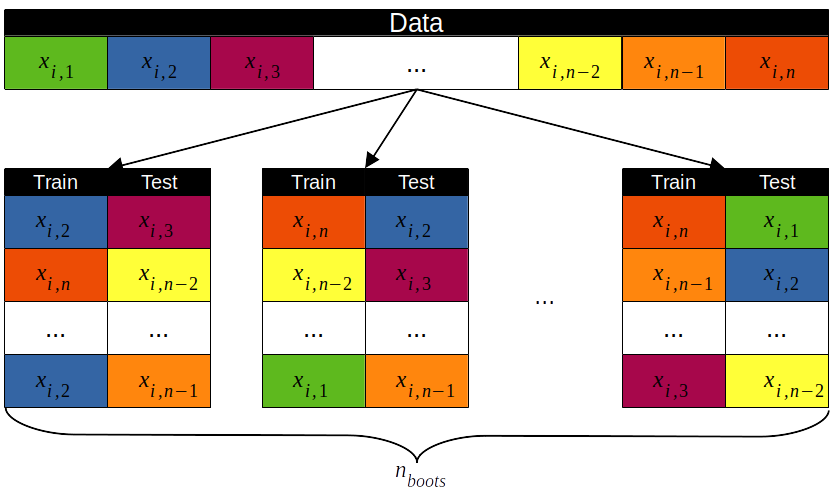
\includegraphics[width=1\linewidth]{Images/bootstrap_diagram.png}
    \caption{Flowchart of the bootstrap algorithm.}
    \label{fig:bootstrap_algorithm}
\end{figure}

\subsubsection{K-fold Cross-Validation}\label{subsubsec:cross_validation}
K-fold cross-validation is an ideal method to circumvent the problem that data is often scarce and there is usually not enough data to set aside a validation set. To avoid this problem the data into $k$ parts of the same size \cite{friedman2001elements}. \newline
The steps of the algorithm are as follows:
\begin{enumerate}
    \item The data is divided into a finite number $k_{folds}$ of equal-sized sets called folds.
    \item For each fold $k_{fi}$:
    \begin{enumerate}
        \item Take the fold as the testing set while the rest of the folds comprise the training set.
        \item Train parameters for the training set and fit them to the testing set.
        \item Compute statistics on the training set: $MSE_i, R^2_i$
    \end{enumerate}
    \item The final statistics of the cross-validation algorithm are the mean of the statistics obtained by considering each fold as the testing set.
\end{enumerate}
\begin{figure}[H]
    \centering
    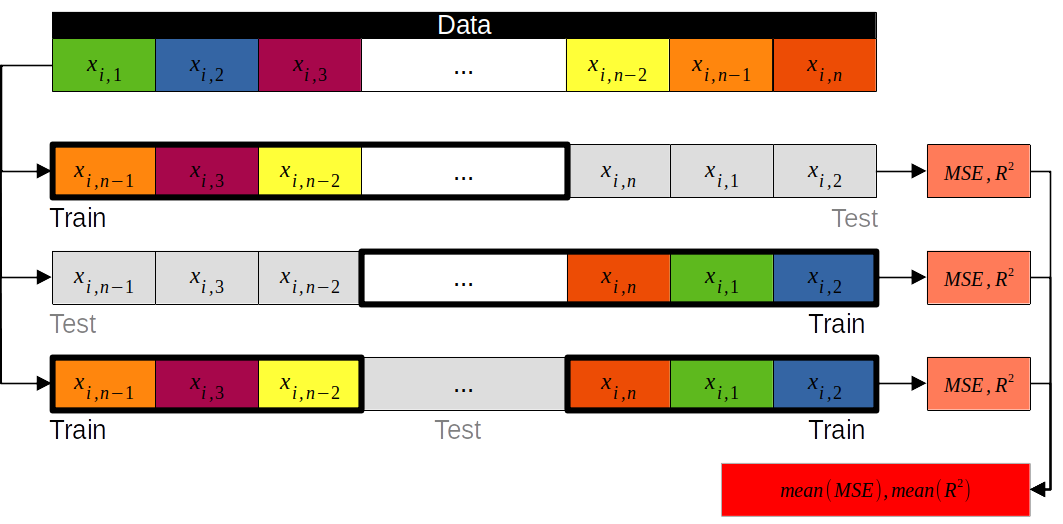
\includegraphics[width=1\linewidth]{Images/cross_validation_diagram.png}
    \caption{Flowchart of the k-fold cross-validation algorithm with $k_{folds}=3$ and $n=9$.}
    \label{fig:cross_val_algorithm}
\end{figure}

%\subsubsection{Stochastic Gradient Descent}\label{subsubsec:SGD}
%SGD is not a machine learning technique but an optimization technique. It is useful in the optimization %requirement for logistic regression. 

%SGD comes in various variants. The most common variant due to its good empirical performance is a mix of epoch and mini-batches. Mini-batches are a subset of data of size m obtained by sampling the whole training data without replacement. This is where randomness and stochasticity come from.
\subsection{Data} \label{subsec:data_linear_regression}
\subsection{Results} \label{subsec:results_linear_regression}

This \href{https://github.com/am-kaiser/CompSci-Project-1/blob/main/regression_analysis/examples/linear_regression_analysis.ipynb}{jupyter notebook} consists of examples to apply different regression techniques. It also consists of widgets where the precalculated statistical performance of different regression methods can be viewed for over a $10^5$ parameter combinations. The data for these experiments is included in the repository. At the end of the jupyter notebook, one can find code that will allow for simulating more parameter combinations if needed. This will overwrite the existing data and also would take a significant time to run. For $10^5$ parameter combinations, it took us about $2$ hours to obtain the data.

\subsubsection{Terminology of symbols and variable names}
Here, we list the names of the variables that are the options in the widgets of the jupyter notebook. The corresponding symbols if applicable are also shown. These symbols relate the variable names to their corresponding mathematical notation used in this report. The general template is the following \\
\\
Symbol: variable name → explanation \\
\\
The list of widget variables are:
\begin{itemize}
    \item $p:$  polynomial order → the order of 2D polynomial used for fitting
    \item $var:$  noise\_var → the variance of the zero mean Gaussian noise added to the Franke data
    \item $r:$  ratio → testing ratio. For example, if the ratio is 0.1 then the test set comprises 10 percent of the dataset.
    \item $n:$  num → the number of points taken along each direction of the input vector. If num = 20, then the total number of data points is 20*20 = 400
    \item stat → Displays the chosen statistic
    \begin{itemize}
        \item $MSE_{train}:$ training MSE
        \item $MSE_{test}:$ testing MSE
        \item ${R^2_{train}}:$ training R2 score
        \item ${R^2_{test}}:$ testing R2 score
        \item $bias_{test}:$ bias in test data
        \item $var_{test}:$ variance in test prediction
    \end{itemize}
    \item method → to choose the regression type
    \begin{itemize}
        \item direct solution and stochastic gradient descent solution available
        \begin{itemize}
            \item OLS
            \item OLS with bootstrap resampling
            \item OLS with cross-validation resampling
            \item Ridge
            \item Ridge with bootstrap resampling
            \item Ridge with cross-validation resampling
        \end{itemize}
        \item direct Solution only (using scikit learn)
        \begin{itemize}
            \item Lasso
            \item Lasso with bootstrap resampling
            \item Lasso with cross-validation resampling
        \end{itemize}
    \end{itemize}
    \item $n_b:$  n\_boot → number of times bootstrap sampling is performed in the bootstrap method. Changing this for methods that doesn't involve bootstrap sampling will not have any effect
    \item $k_f:$  k\_fold → number of folds in the cross-validation method. Changing this for methods that doesn't involve cross-validation will not have any effect
    \item $\lambda_r:$  ridge\_lambda → regularisation parameter for ridge regression
    \item $\lambda_l:$ lasso\_lambda → regularisation parameter for LASSO regression
    \item $\eta:$ learn\_rates → parameter that controls the descent jump size in gradient descent methods
    \item $n_e:$ epoch → parameter that controls the number of times the algorithm works through the entire dataset in gradient descent methods
    \item $n_{batch}:$ number of batches → parameter that controls the mini-batch size in gradient descent methods
\end{itemize}

\subsubsection{Ordinary Least Squares (OLS)}

Here, we present selected results of linear regression that we find particularly interesting.

Foremost, we look at the $MSE_{train}$ of OLS (see figure \ref{fig:ols1}). We see that the $MSE_{train}$ reduces as the model complexity or polynomial order($p$) increases. In other words, with increasing complexity, our model becomes more \textcolor{red}{flexible. Is that the right word?} As the input data is an exponential function that can be expressed as a series of polynomials, increasing the terms in the fitted polynomial should decrease the $MSE_{train}$. We also see that for large values of test ratio, i.e. $r = 0.4$, and low number of data points, $n = 100$, which amounts to about $60$ data points in the training set, the $MSE_{train}$ is significantly lower for high $p$.

\begin{figure}[htb]
\centering
\begin{subfigure}{.5\textwidth}
  \centering
  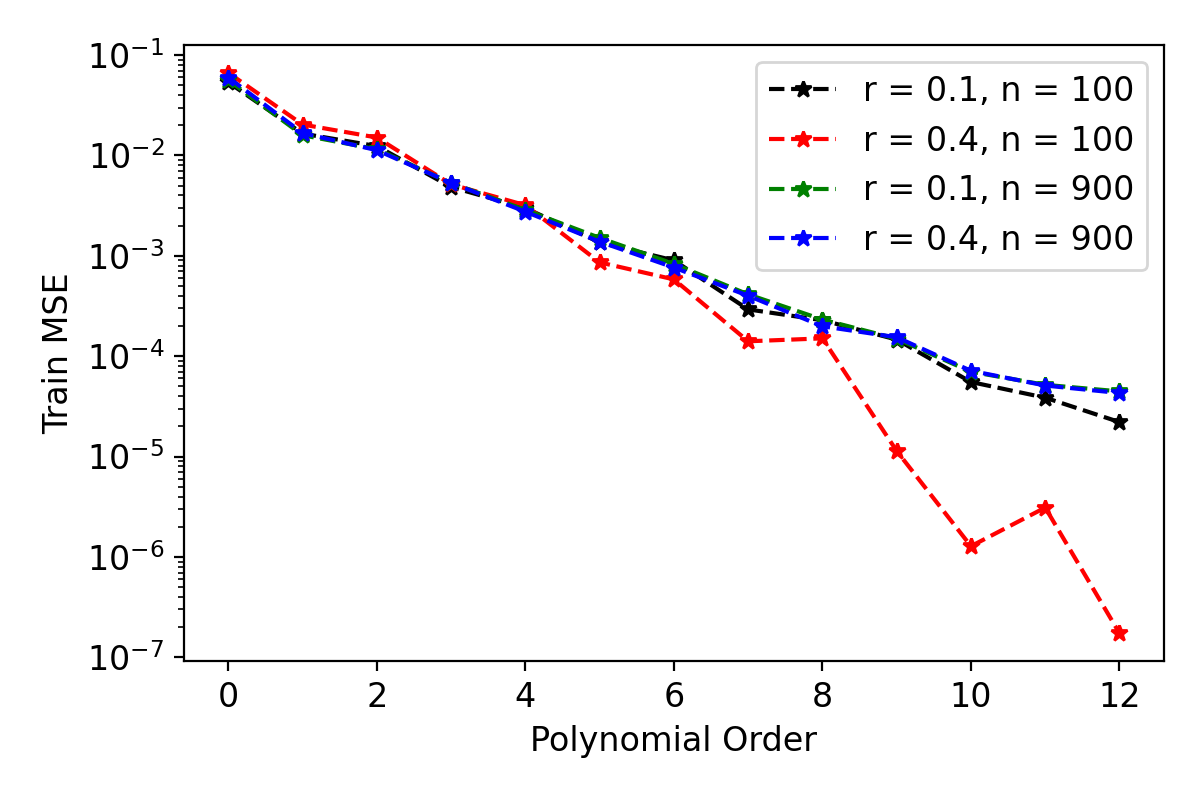
\includegraphics[width=.9\linewidth]{Images/ols2.png}
  \caption{}
  \label{fig:ols1}
\end{subfigure}%
\begin{subfigure}{.5\textwidth}
  \centering
  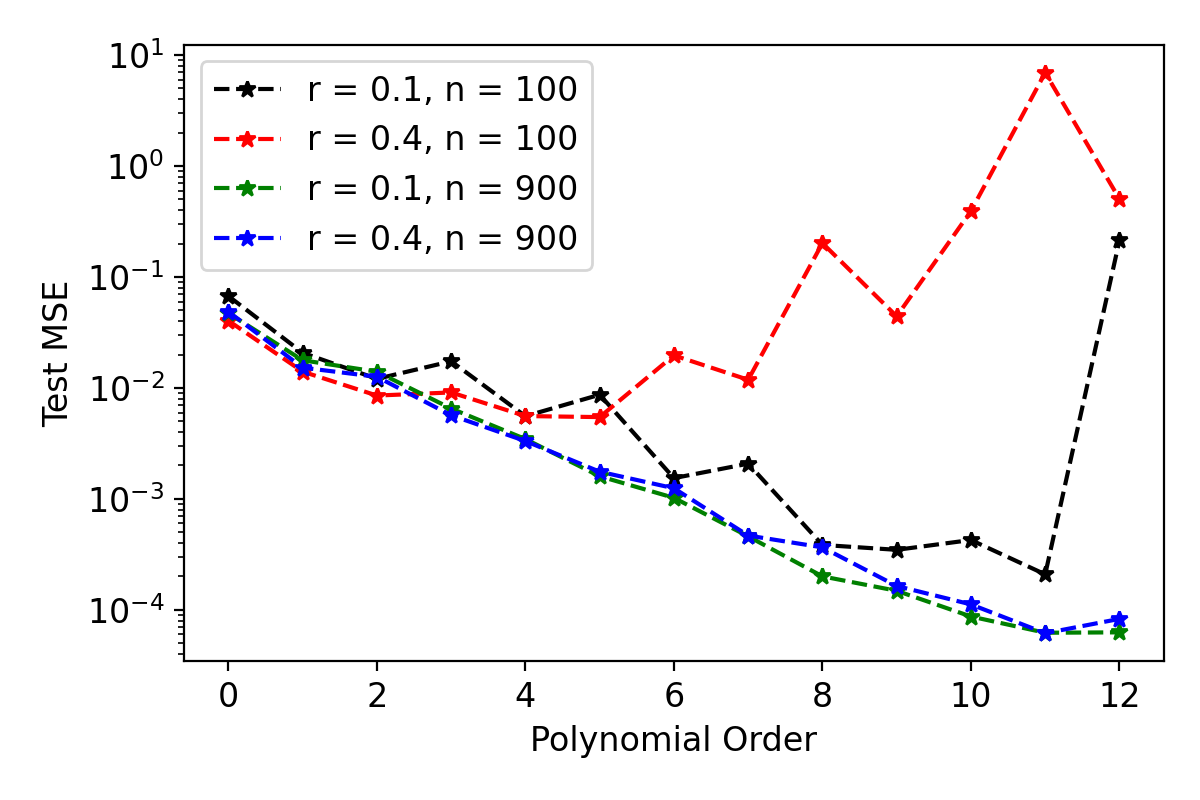
\includegraphics[width=.9\linewidth]{Images/ols1.png}
  \caption{}
  \label{fig:ols2}
\end{subfigure}
\begin{subfigure}{.5\textwidth}
  \centering
  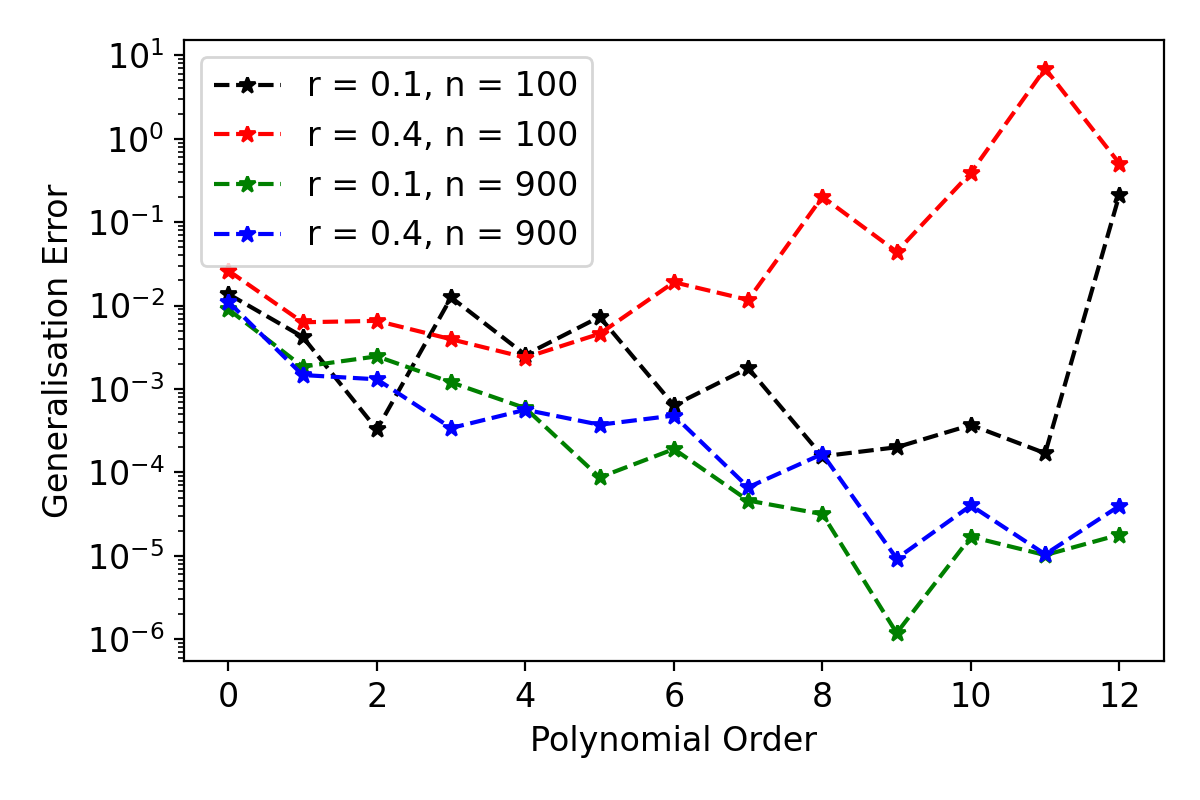
\includegraphics[width=.9\linewidth]{Images/ols3.png}
  \caption{}
  \label{fig:ols3}
\end{subfigure}
\begin{subfigure}{.45\textwidth}
  \centering
  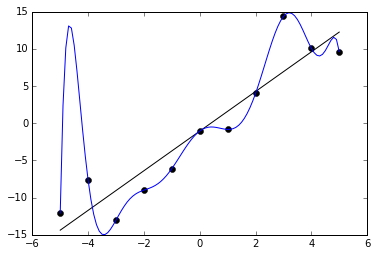
\includegraphics[width=.9\linewidth]{Images/Overfitted_Data.png}
  \caption{}
  \label{fig:overfit}
\end{subfigure}
\caption{OLS for noiseless Franke data: (a) $MSE_{train}$, (b) $MSE_{test}$ and (c) Generalization error plotted as functions of model complexity. (d) Schematic describing overfitting of data due to higher model complexity (Source: Ghiles, Wikipedia). }
\label{fig:OLS1}
\end{figure}

Now, if we shift attention to the $MSE_{test}$, we see that for r=0.4, n=100, the generalization is poor (see figure \ref{fig:ols2}). This is the result of overfitting. This also happens for r=0.1, n=100 albeit not as strongly. This shows that even for low values of $MSE_{train}$, the model can perform poorly. We see that if the number of datapoints is higher in the training set, then there is no overfitting. This is also evident by looking at the generalization error(see figure \ref{fig:ols3}). The model 'sees' more variety of data during the training phase which prevents it from overfitting. Provided we don't overfit, the $MSE_{test}$ reduces as p  increases. It should be noted that irrespective of the number of data points used for training, there exist p's where we will experience overfitting. The figure \ref{fig:overfit} shows a 1D polynomial with order equal to the number of points will perform much worse than a linear polynomial for unseen data. If $n_{train}$ is the number of training data points then to prevent overfitting in many situations, we need $n_{train} >> p$. 

Next, we see that the introduction of noise into the dataset increases $MSE_{train}$ (see figure \ref{fig:ols4}). We also see that introducing noise affects the $MSE_{test}$ of a dataset with a larger number of points significantly when model complexity is high (see figure \ref{fig:ols5}). $MSE_{test}$ decreases initially with model complexity but later plateaus. This portrays that the higher degree of freedom, introduced by additional polynomial terms, doesn't sufficiently capture the noise. When the model complexity is low, the prediction is unaffected by the presence of noise. 

\begin{figure}[htb]
\centering
\begin{subfigure}{.5\textwidth}
  \centering
  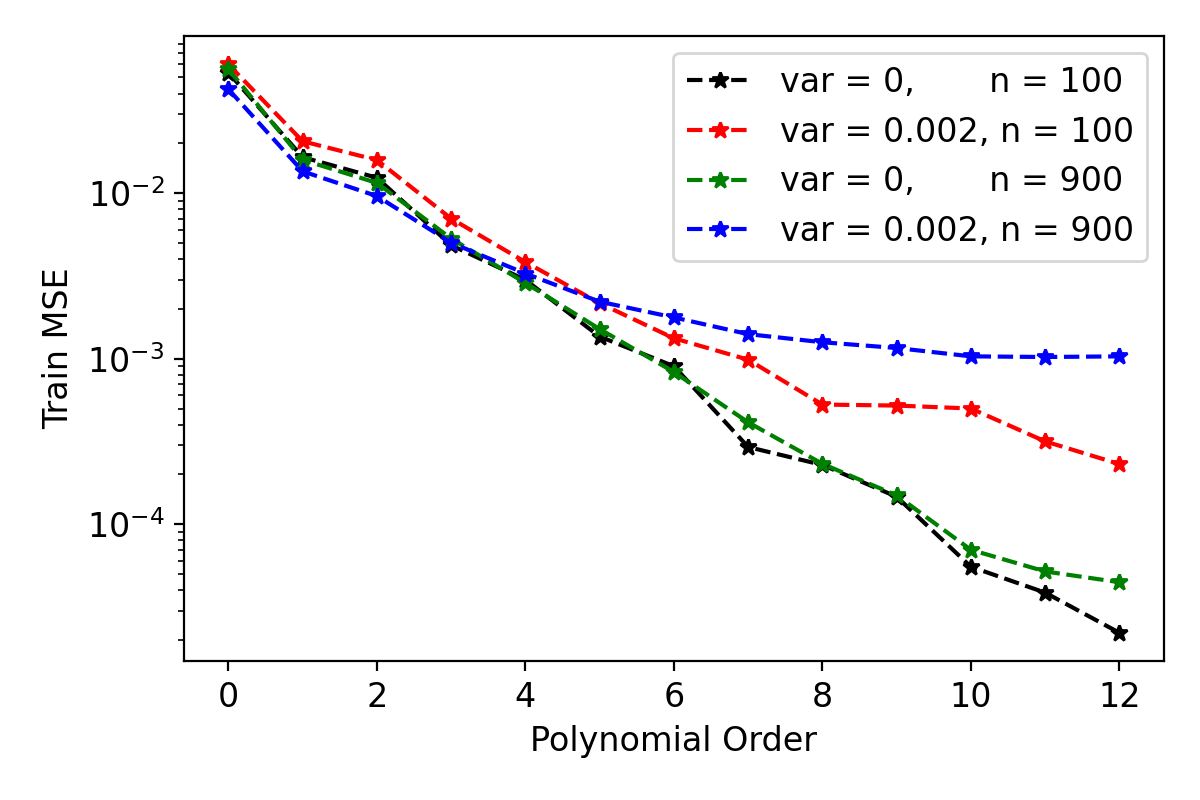
\includegraphics[width=.9\linewidth]{Images/ols5.png}
  \caption{}
  \label{fig:ols4}
\end{subfigure}%
\begin{subfigure}{.5\textwidth}
  \centering
  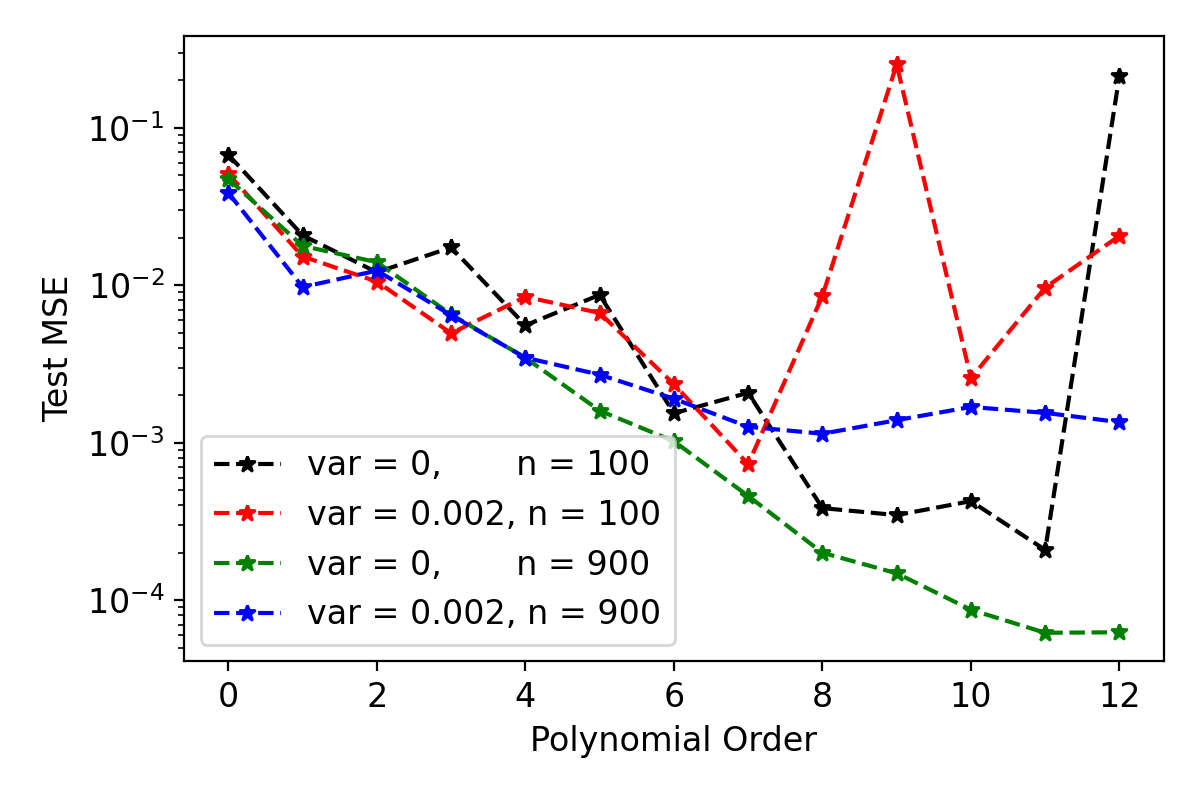
\includegraphics[width=.9\linewidth]{Images/ols4.png}
  \caption{}
  \label{fig:ols5}
\end{subfigure}
\caption{OLS for $r=0.1$ and $n=900$: (a) $MSE_{train}$ and (b) $MSE_{test}$ plotted as functions of model complexity}
\label{fig:OLS2}
\end{figure}

\begin{figure}[htb]
\centering
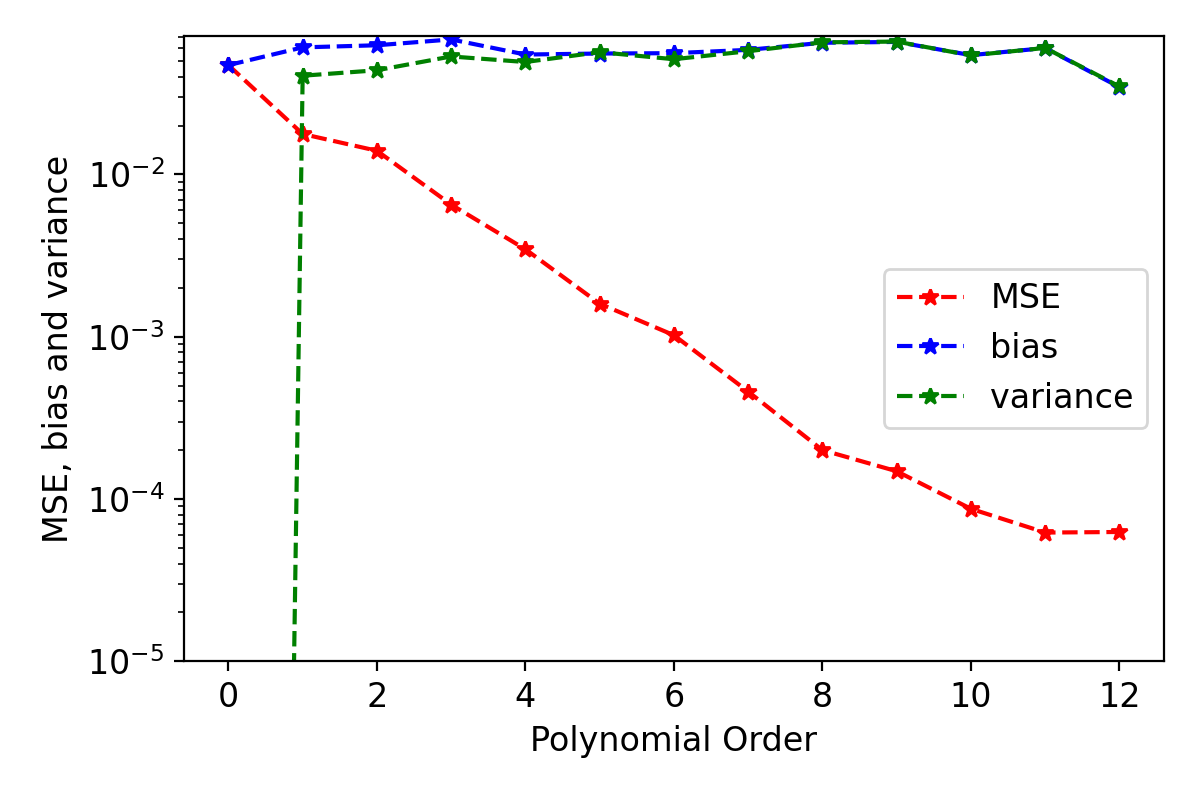
\includegraphics[width=.7\linewidth]{Images/ols7.png}
\caption{OLS for $r=0.1$, $var=0$ and $n=900$. Bias and variance plotted as functions of model complexity}
\label{fig:OLS3}
\end{figure}

If we now look at the bias and variance, they are both roughly constant as the model complexity increases (see figure \ref{fig:OLS3}). This might be a discrepancy in our calculation and it prevents us from understanding the bias-variance tradeoff. This behavior is observed even when other parameters are changed. As variance measures, the spread of our prediction, and the plots show that our model always has a finite spread. As bias is a measure of the mean deviation of our prediction from the truth, the constant values raise questions on our calculations. We know that parameters like $r$, $var$, $p$ and $n$ have an impact on the $MSE_{test}$, but as the bias seems to be roughly the same then that shows that irrespective of the parameters, our model has approximately the same mean value of the predicted output. Either our model is capturing the mean well almost always or our calculations of bias and variance are incorrect.

\subsubsection{Ridge and LASSO Regression}
In ridge regression, we use the $L_2$ norm of the parameter vector $\boldsymbol \beta$ as a penalty term. As we are not tuning the size of the elements of the design matrix, the interrelations between the different columns should remain the same. This is the case when the design matrix is orthogonal. As we use polynomials as basis functions, the columns of the design matrix are likely to be independent. They will not be independent if there is a correlation between $x_{i1}$ and $x_{i2}$ which is not true in our dataset. So, the parameters in ridge regression would be rescaled by a factor of $\frac{1}{1+\lambda_r}$ compared to the OLS parameters \cite{mehta2019high}. However, since that there might be errors in calculating the pseudoinverse, the scaling might not always be by the factor of $\frac{1}{1+\lambda_r}$. So, not all parameters are scaled the same. This would deviate the predictions from that of the OLS. We can see this in the figure \ref{fig:ridge7} and \ref{fig:ridge7b} where the regularisation parameter affects both the training and prediction phase. The training and testing error both worsen as $\lambda_r$ increases. The deviation from the OLS errors kicks in at a lower model complexity for higher values of  $\lambda_r$. For lower model complexity, the ridge regression performs similarly to OLS. But, as the complexity increases, ridge regression has a poorer prediction. It is unclear why this happens, but the most likely reason might be numeric underflow or overflow. 



\begin{figure}[htb]
\centering
\begin{subfigure}{.5\textwidth}
  \centering
  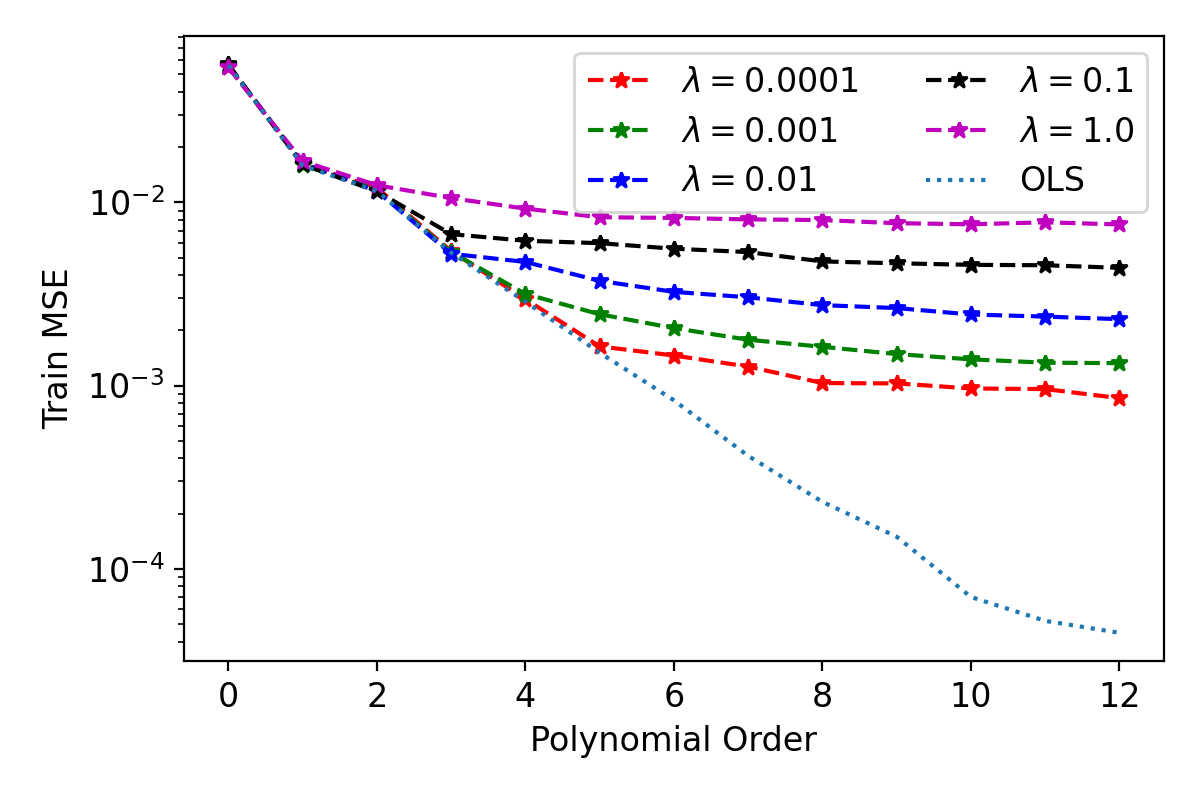
\includegraphics[width=.9\linewidth]{Images/ridge7b.png}
  \caption{}
  \label{fig:ridge7}
\end{subfigure}%
\begin{subfigure}{.5\textwidth}
  \centering
  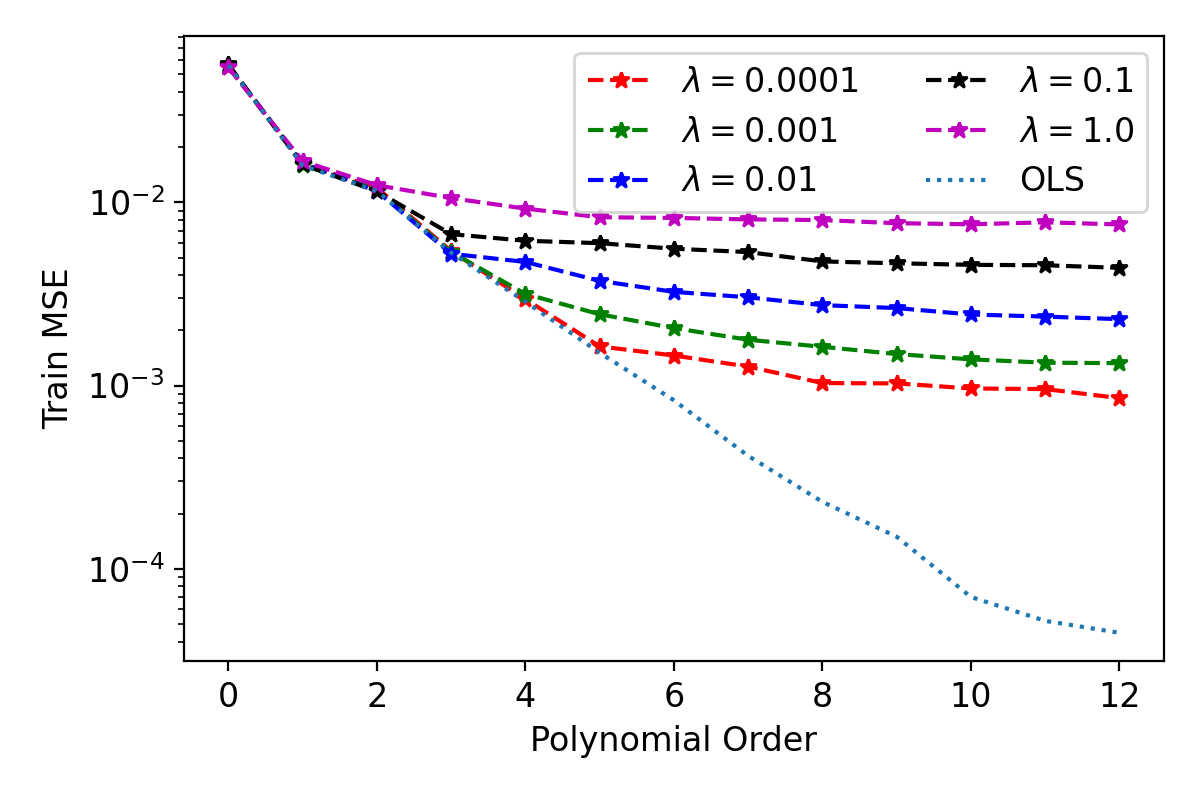
\includegraphics[width=.9\linewidth]{Images/ridge7b.png}
  \caption{}
  \label{fig:ridge7b}
\end{subfigure}
\caption{Ridge regression for $r=0.1$, $var=0$ and $n=900$: (a) $MSE_{train}$ and (b) $MSE_{test}$ plotted as functions of model complexity for different regularisation strength}
\label{fig:Ridge1}
\end{figure}

Meanwhile, in LASSO regression, we use the $L_1$ norm of the parameter vector $\boldsymbol \beta$ as a penalty term. Visually, this is equivalent to optimizing the parameters until we hit the edges of a constraint hypercuboid. While, in ridge regression, we hit the surface of a constraint hyperellipsoid. See chapter 3 of \cite{friedman2001elements} for more details. This means that in LASSO regression when the optimum parameters are reached, the components of some of the parameter vector $\boldsymbol \beta$ are 0. These features were not important enough in affecting the combined optimization of the least square error and the $L_1$ norm of the parameter vector $\boldsymbol \beta$. We see in the figure \ref{fig:lasso7} that both the training error and testing error worsen as the $\lambda_l$ increases. But, the performance is much worse than for ridge regression and is several orders of magnitude worse than OLS. As $\lambda_l$ increases, more components of $\boldsymbol \beta$ turn out to be 0. 


\begin{figure}[htb]
\centering
\begin{subfigure}{.5\textwidth}
  \centering
  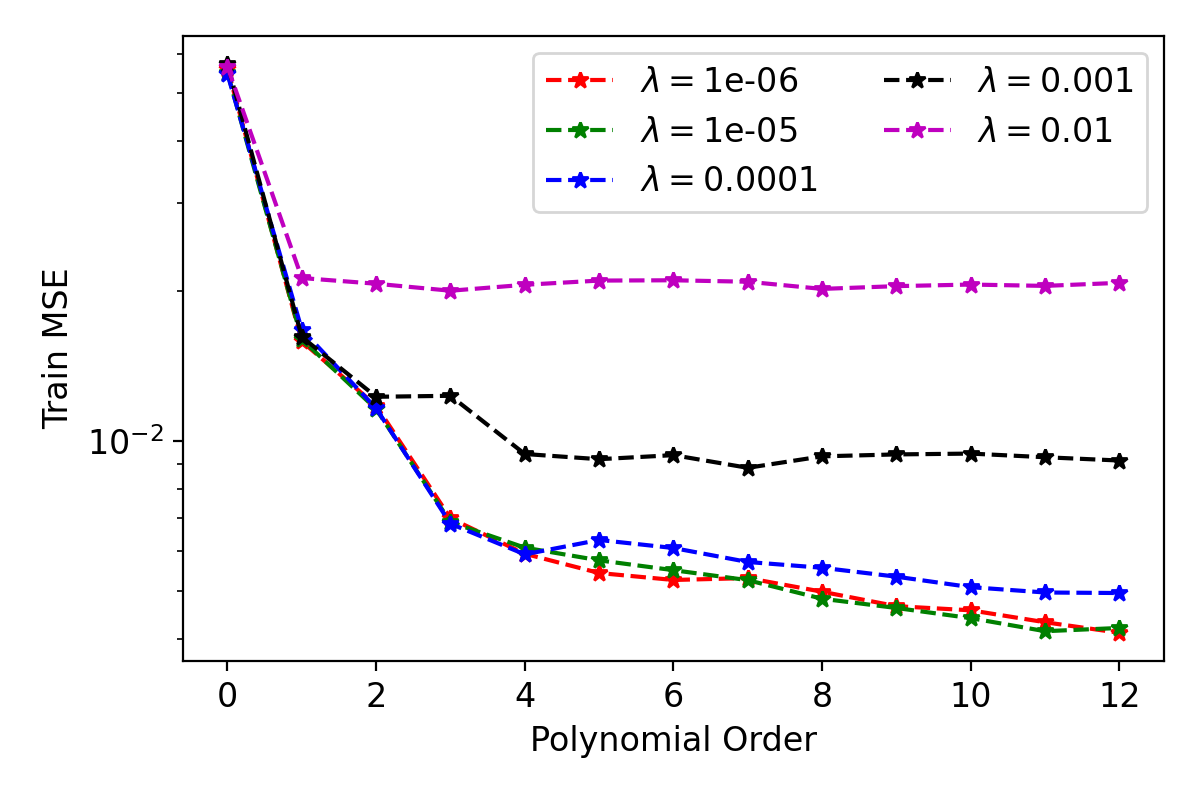
\includegraphics[width=.9\linewidth]{Images/lasso7b.png}
  \caption{}
  \label{fig:lasso7}
\end{subfigure}%
\begin{subfigure}{.5\textwidth}
  \centering
  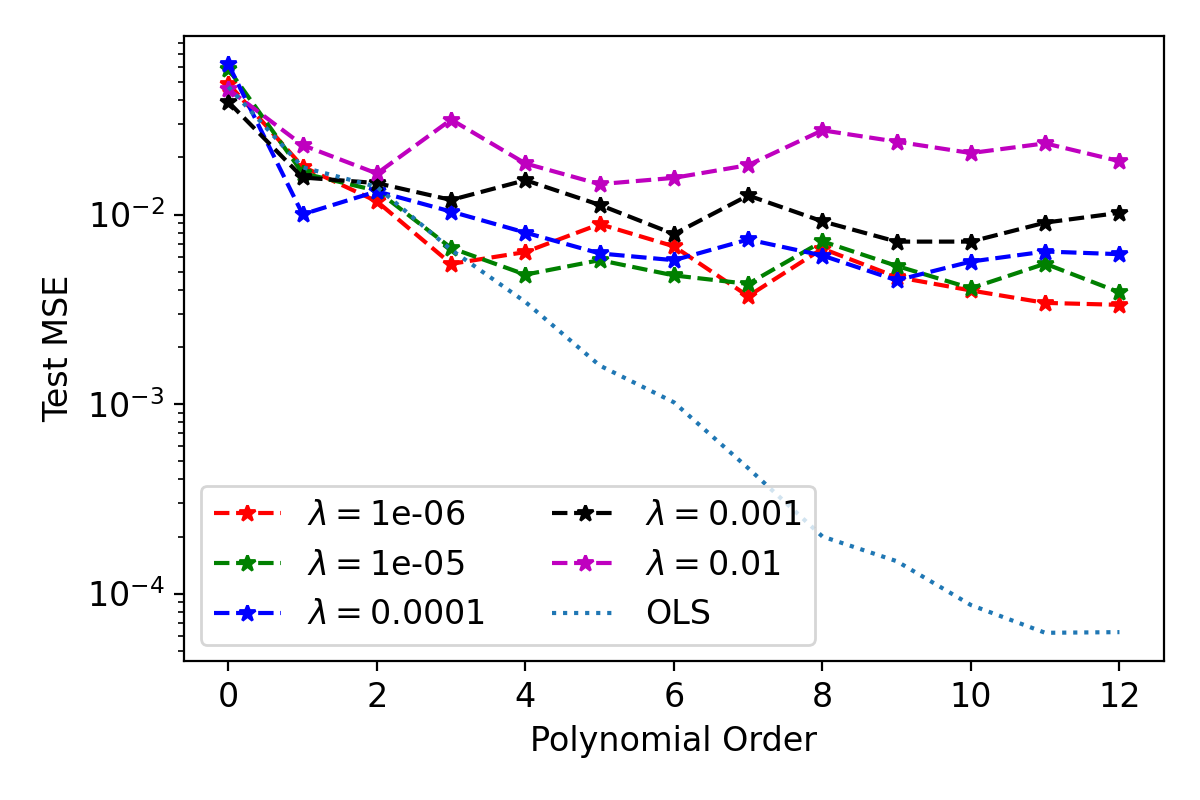
\includegraphics[width=.9\linewidth]{Images/lasso7.png}
  \caption{}
  \label{fig:lasso7b}
\end{subfigure}
\caption{LASSO regression for $r=0.1$, $var=0$ and $n=900$: (a) $MSE_{train}$ and (b) $MSE_{test}$ plotted as functions of model complexity for different regularisation strength}
\label{fig:Lasso1}
\end{figure}

\begin{figure}[htb]
\centering
\begin{subfigure}{.5\textwidth}
  \centering
  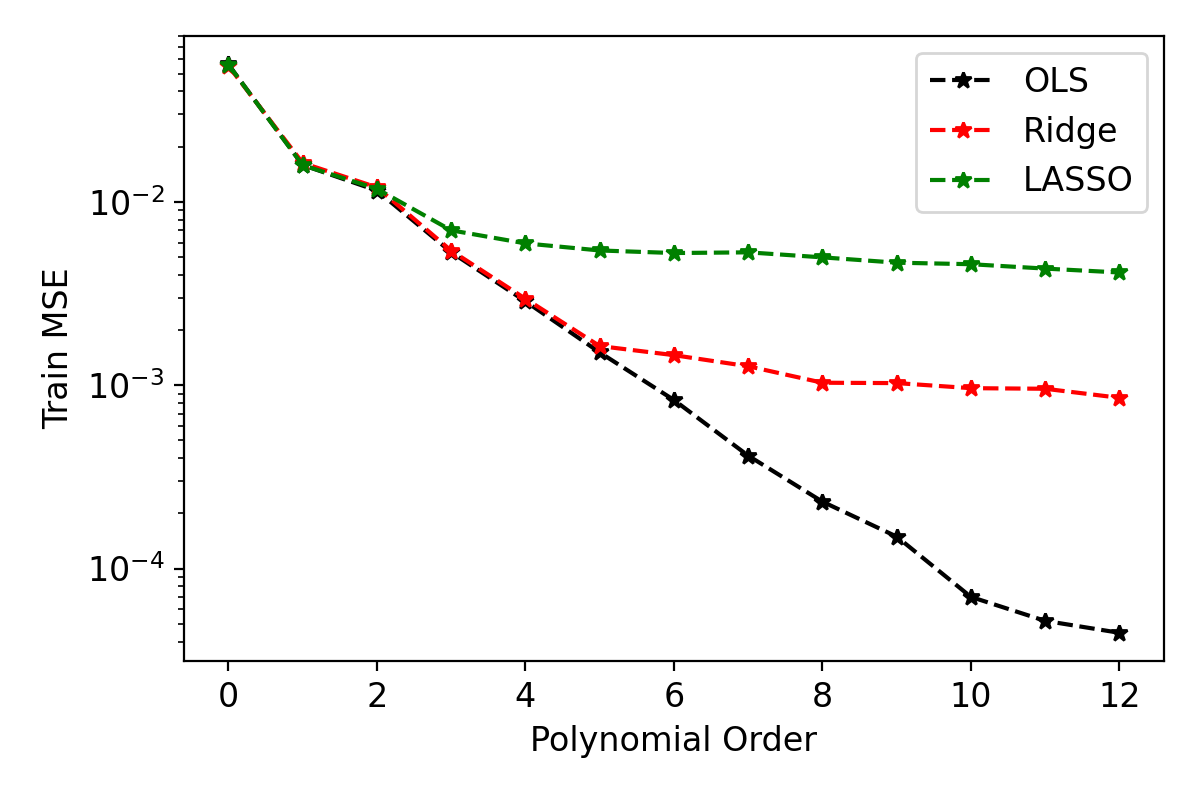
\includegraphics[width=.9\linewidth]{Images/orl2.png}
  \caption{}
  \label{fig:orl1}
\end{subfigure}%
\begin{subfigure}{.5\textwidth}
  \centering
  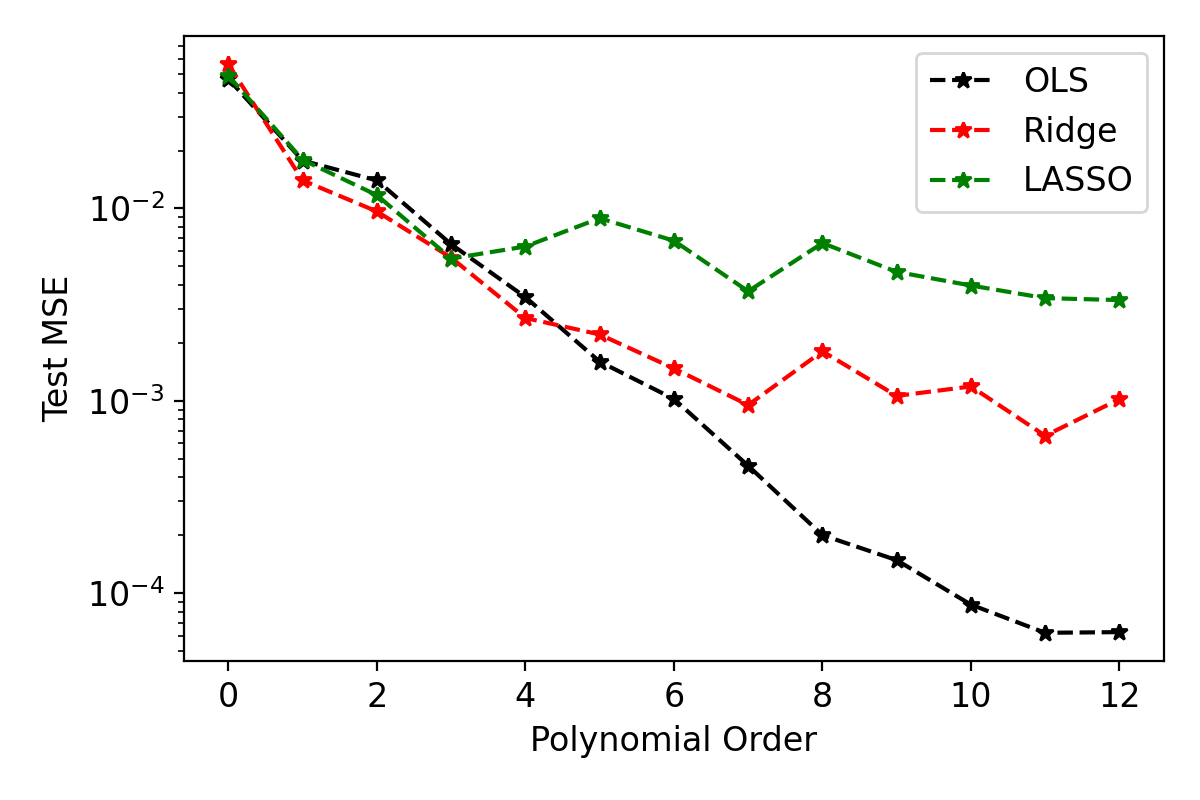
\includegraphics[width=.9\linewidth]{Images/orl1.png}
  \caption{}
  \label{fig:orl2}
\end{subfigure}
\begin{subfigure}{.5\textwidth}
  \centering
  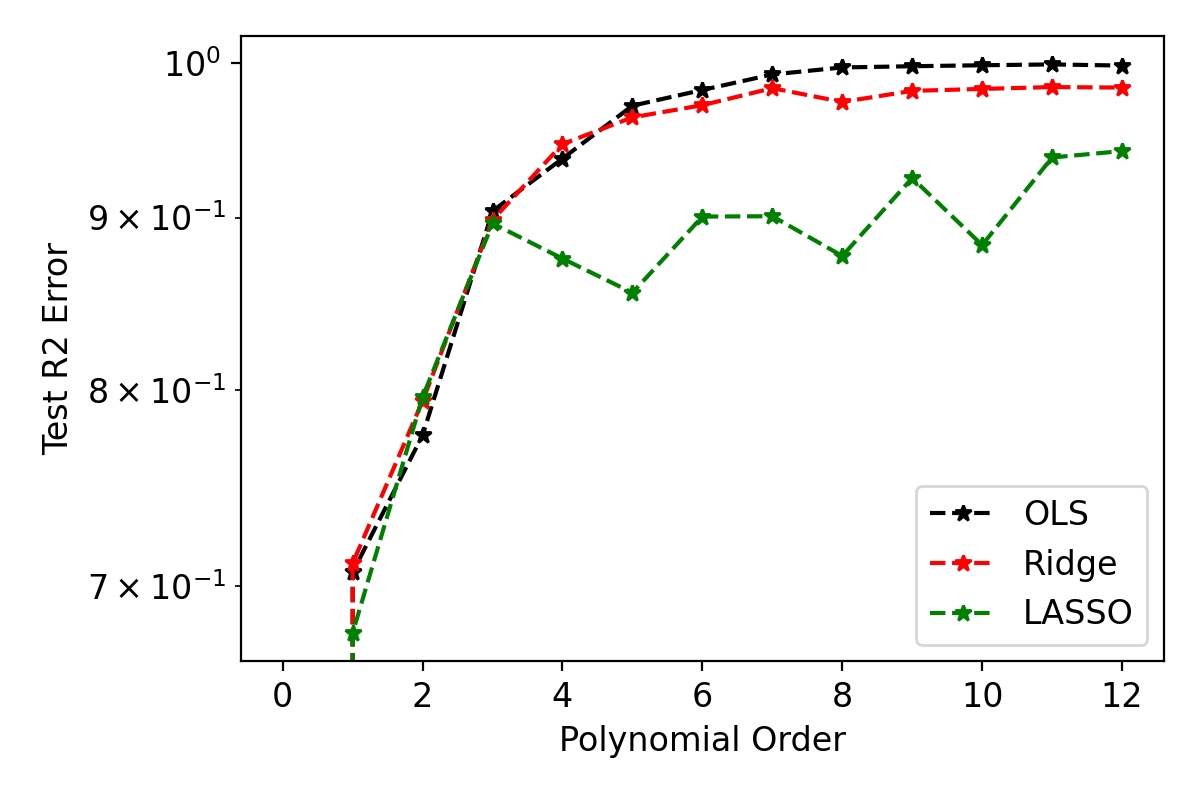
\includegraphics[width=.9\linewidth]{Images/orl3.png}
  \caption{}
  \label{fig:orl3}
\end{subfigure}
\caption{OLS, Ridge($\lambda_r = \num{1e-4}$) and LASSO($\lambda_l = \num{1e-6}$) regression for $r=0.1$, $var=0$ and $n=900$: (a) $MSE_{train}$, (b) $MSE_{test}$ and (c) $R^2_{test}$ plotted as functions of model complexity}
\label{fig:ORL1}
\end{figure}

The figure \ref{fig:orl1} and \ref{fig:orl2} show the relative performance in training and testing for OLS, Ridge and LASSO regression. Here, we show the best-case scenario for Ridge and LASSO among the parameters screened by us. OLS outperforms Ridge regression by an order of magnitude while it is 2 orders of magnitude better than LASSO. This is explained by the fact that in OLS, the optimization involves lowering the squared error but in the other methods, there is an additional cost incurred for the size of components of parameter vectors The figure \ref{fig:orl3} shows the $R^2_{test}$ error which is a measure of the variance captured by our model in relation to the actual variance. We see that as the model complexity increases, the $R^2_{test}$ tends to reach 1 for both OLS and Ridge regression. While in LASSO regression, the variance capture is much poorer. Certainly, the results here indicate that OLS performs much better than Ridge and LASSO. Why would these two methods remain relevant? This is because there can be situations where the size of components of $\boldsymbol \beta$ can cause a numerical overflow. Additionally, shrinkage methods like Ridge and LASSO reduce the prediction variability in many situations \cite{friedman2001elements}.

\subsubsection{Regression with Bootstrap and Cross-validation}
\begin{figure}[ht]
\centering
\begin{subfigure}{.5\textwidth}
  \centering
  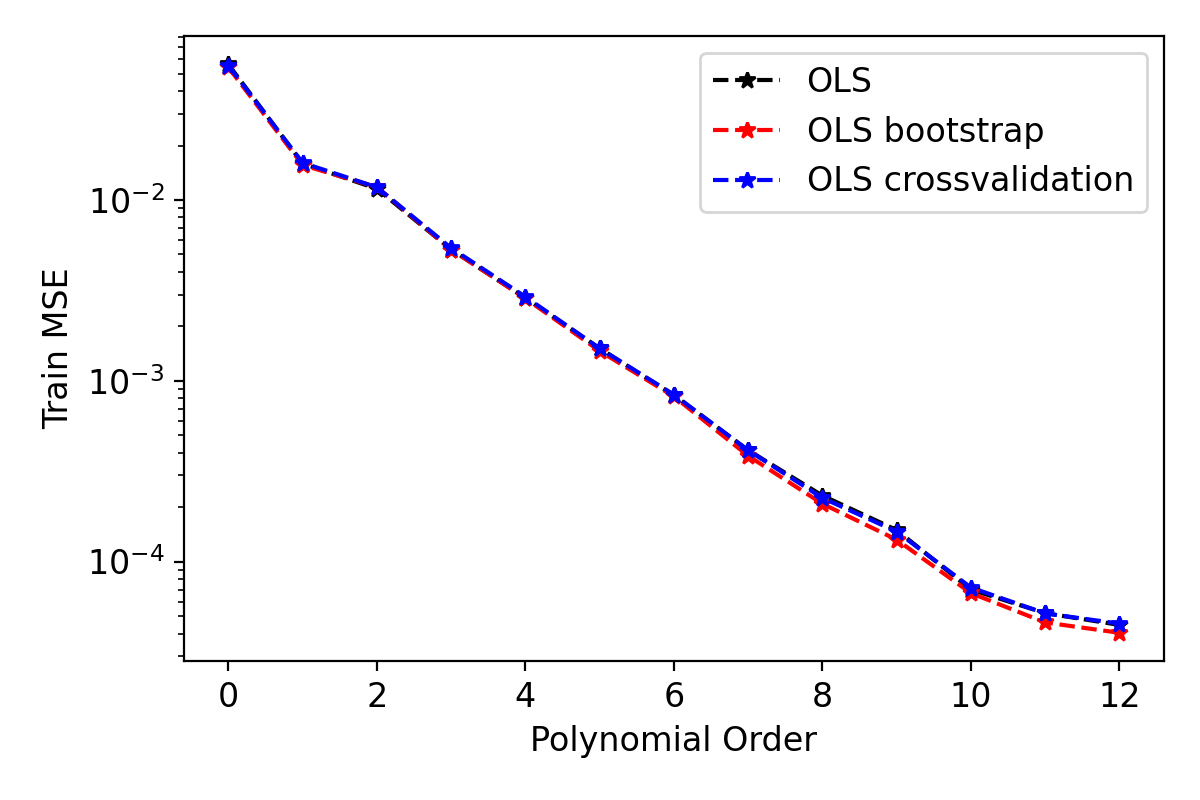
\includegraphics[width=.8\linewidth]{Images/ols9.png}
  \caption{}
  \label{fig:ols9}
\end{subfigure}%
\begin{subfigure}{.5\textwidth}
  \centering
  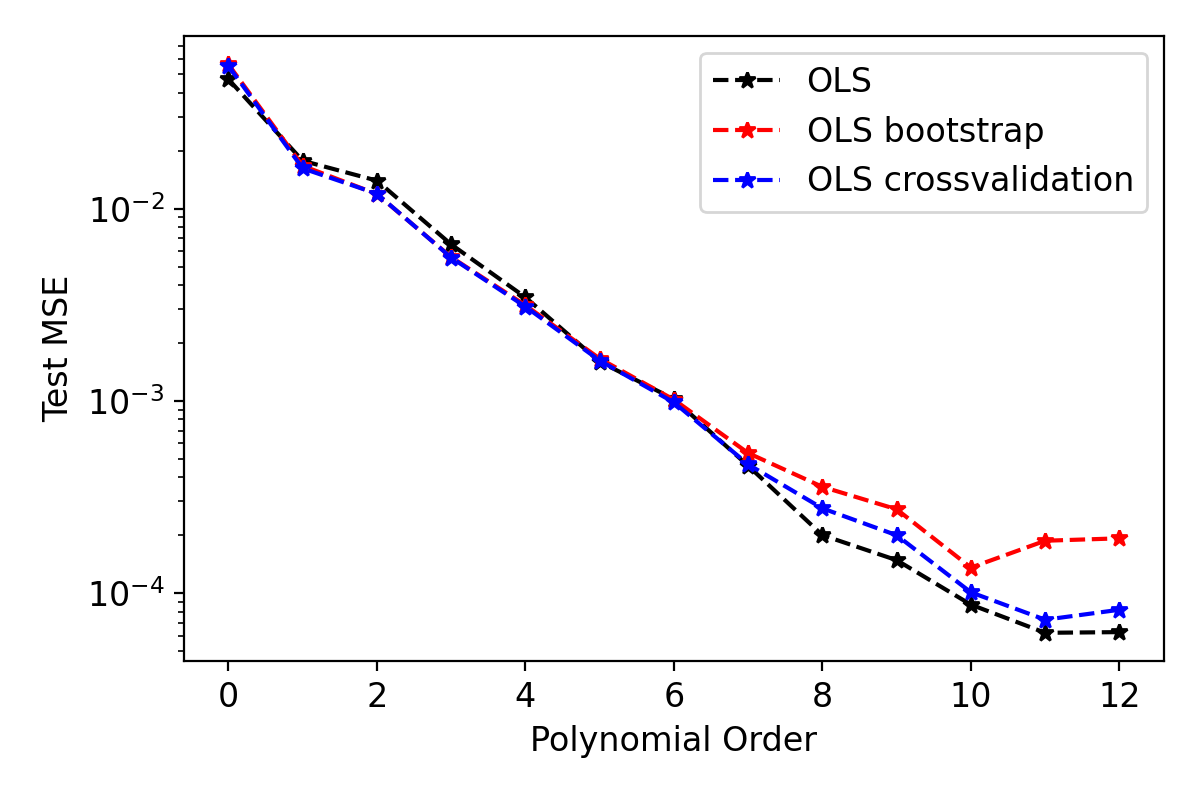
\includegraphics[width=.8\linewidth]{Images/ols8.png}
  \caption{}
  \label{fig:ols8}
\end{subfigure}
\begin{subfigure}{.5\textwidth}
  \centering
  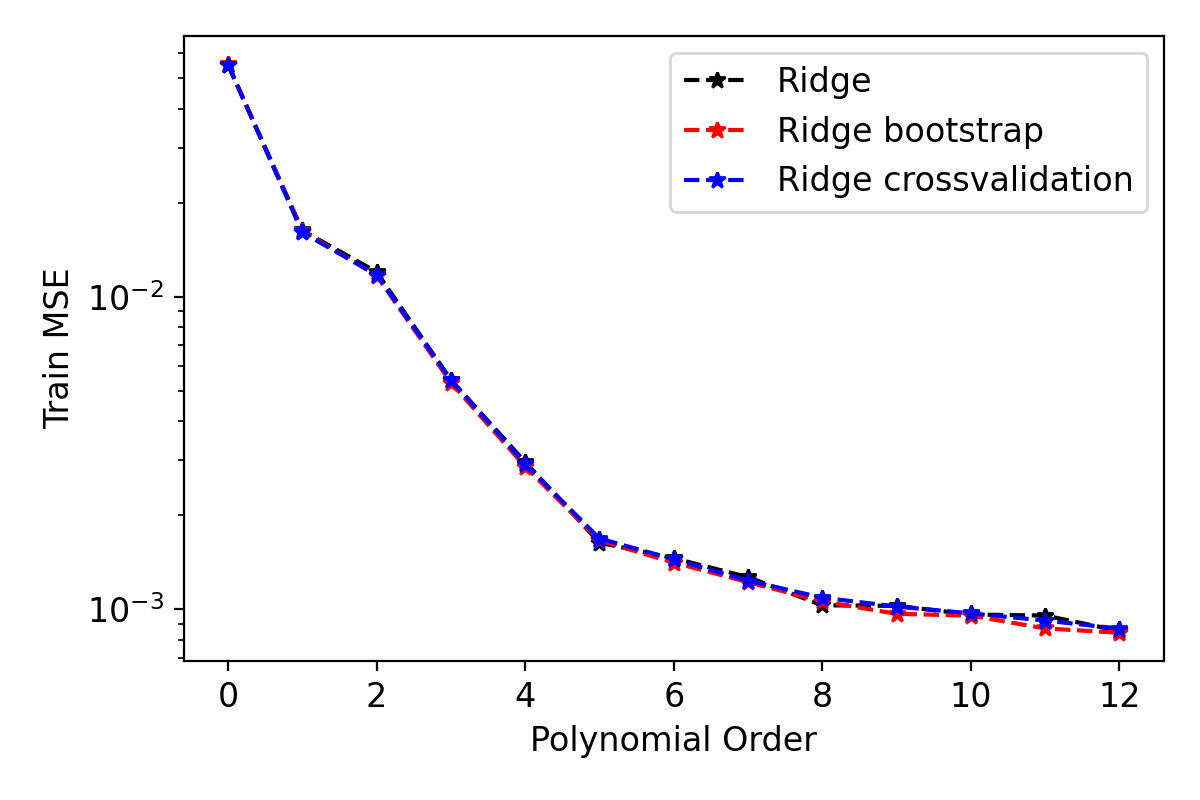
\includegraphics[width=.8\linewidth]{Images/ridge9.png}
  \caption{}
  \label{fig:ridge9}
\end{subfigure}%
\begin{subfigure}{.5\textwidth}
  \centering
  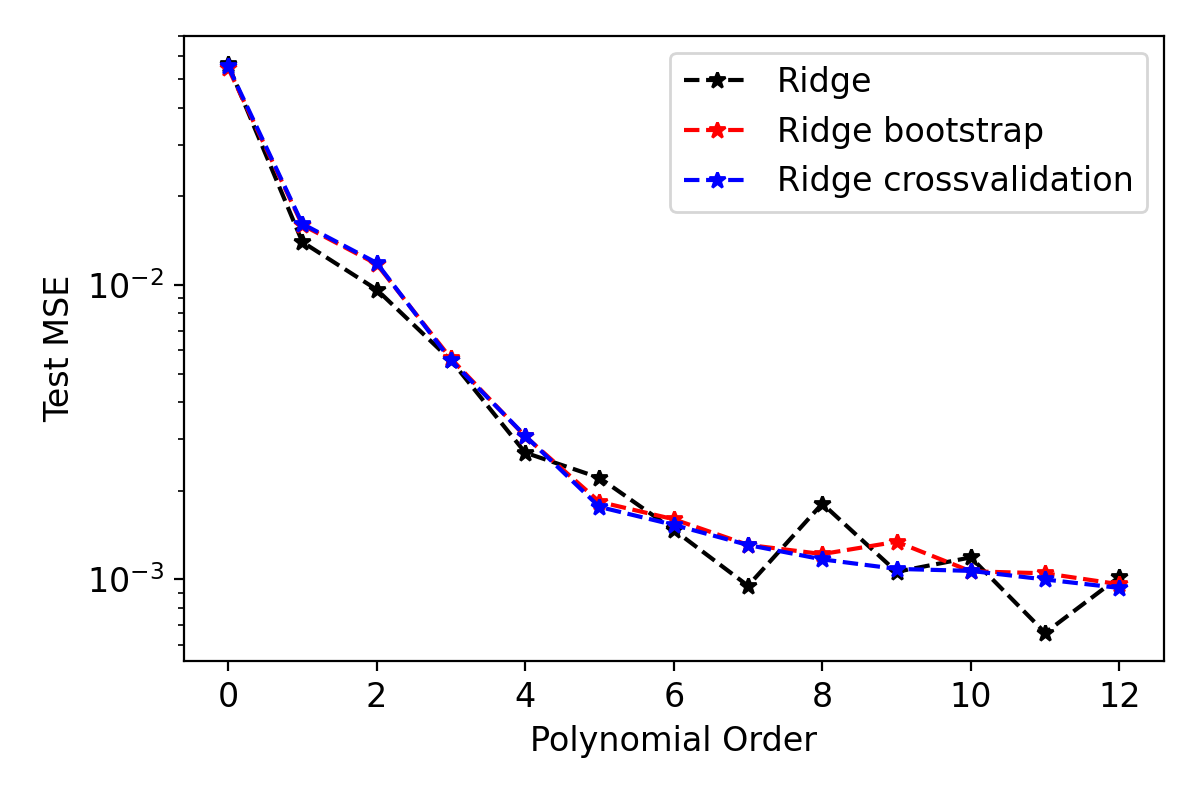
\includegraphics[width=.8\linewidth]{Images/ridge8.png}
  \caption{}
  \label{fig:ridge8}
\end{subfigure}
\begin{subfigure}{.5\textwidth}
  \centering
  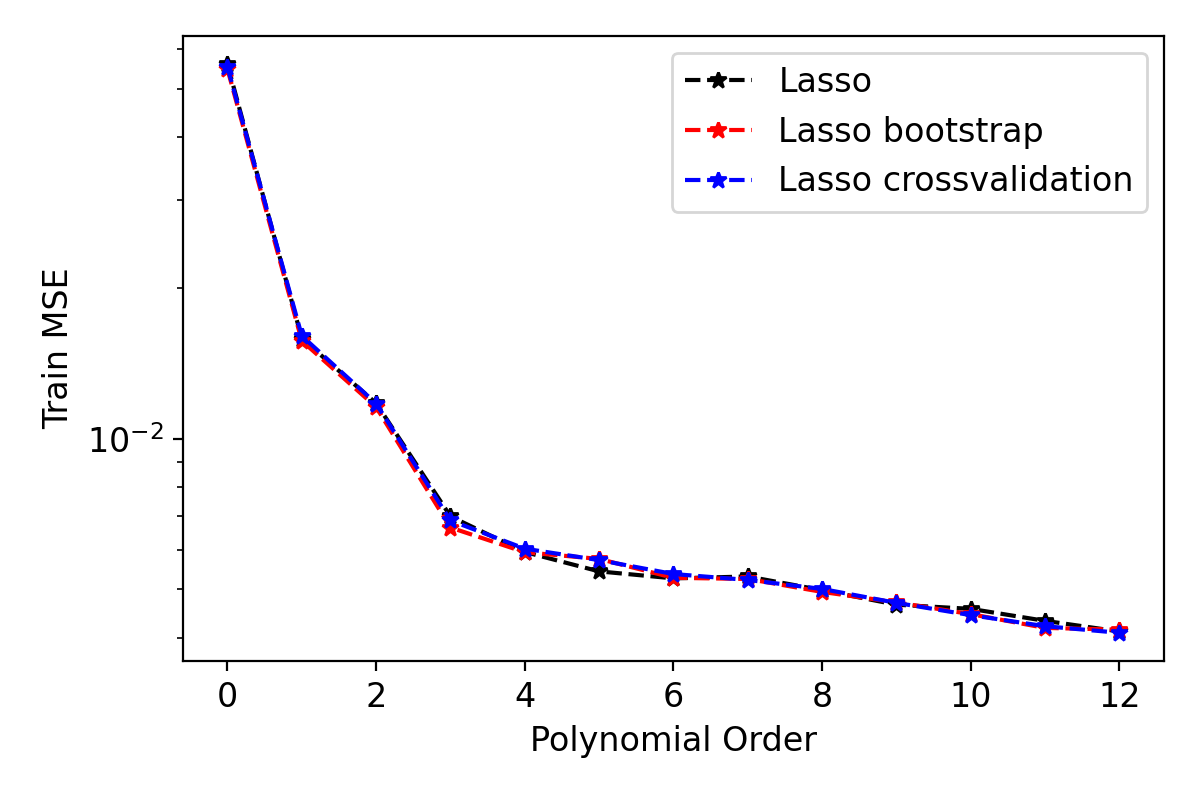
\includegraphics[width=.8\linewidth]{Images/lasso9.png}
  \caption{}
  \label{fig:lasso9}
\end{subfigure}%
\begin{subfigure}{.5\textwidth}
  \centering
  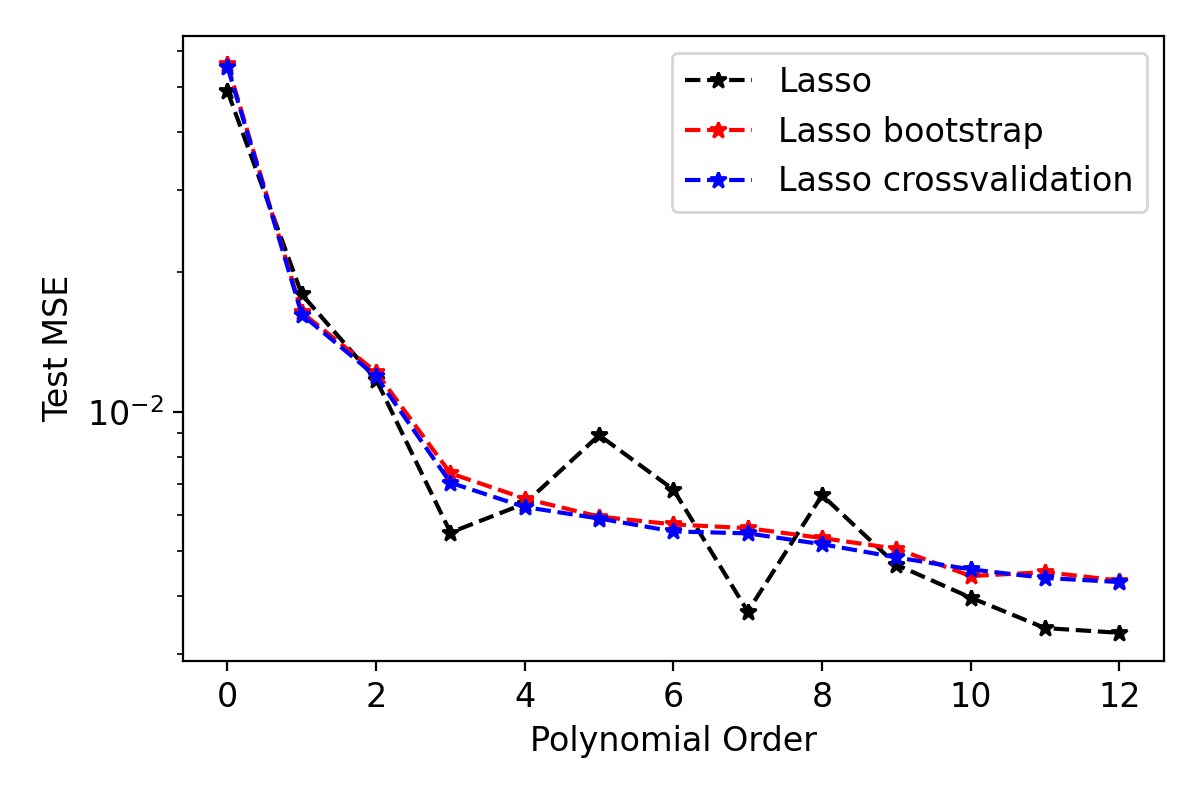
\includegraphics[width=.8\linewidth]{Images/lasso8.png}
  \caption{}
  \label{fig:lasso8}
\end{subfigure}
\caption{For $r=0.1$, $var=0$ and $n=900$: (a), (c), (e) $MSE_{train}$ and  (b), (d), (f) $MSE_{test}$ plotted as functions of model complexity}
\label{fig:OLS_resample}
\end{figure}


\begin{figure}[h!]
\centering
\begin{subfigure}{.5\textwidth}
  \centering
  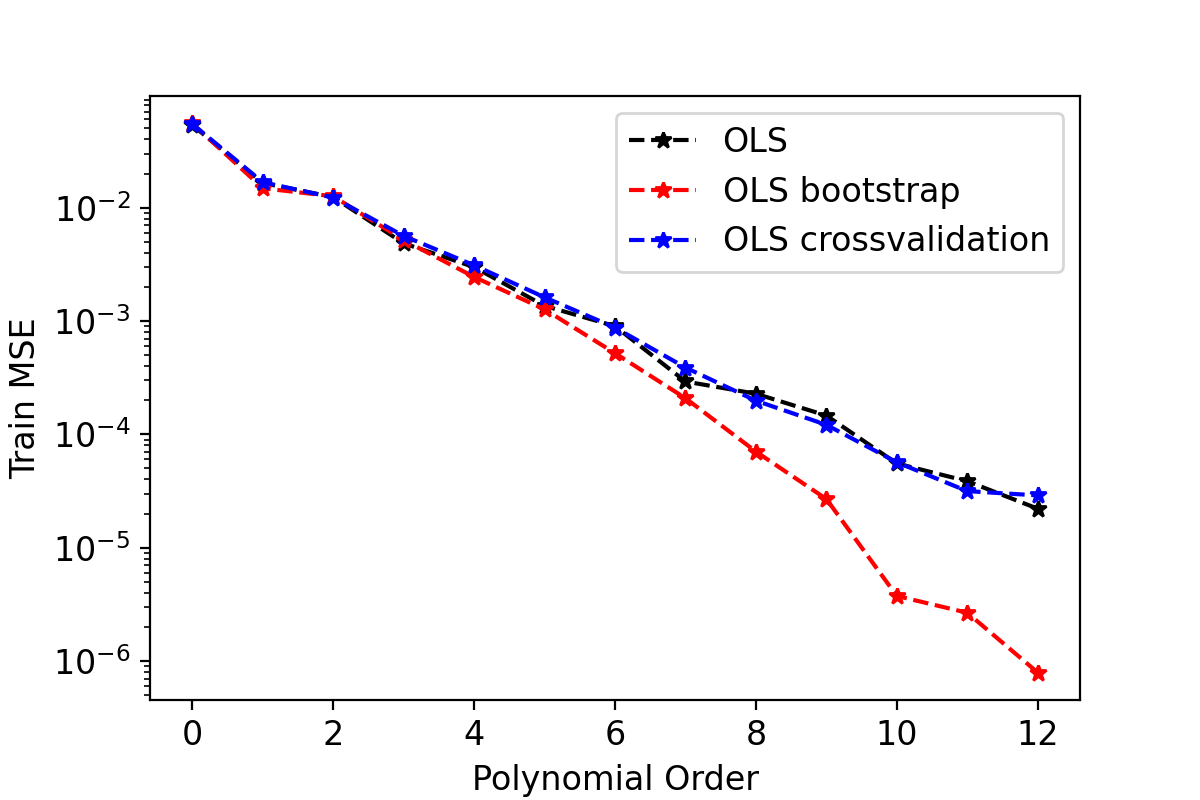
\includegraphics[width=.8\linewidth]{Images/ols15.png}
  \caption{}
  \label{fig:ols15}
\end{subfigure}%
\begin{subfigure}{.5\textwidth}
  \centering
  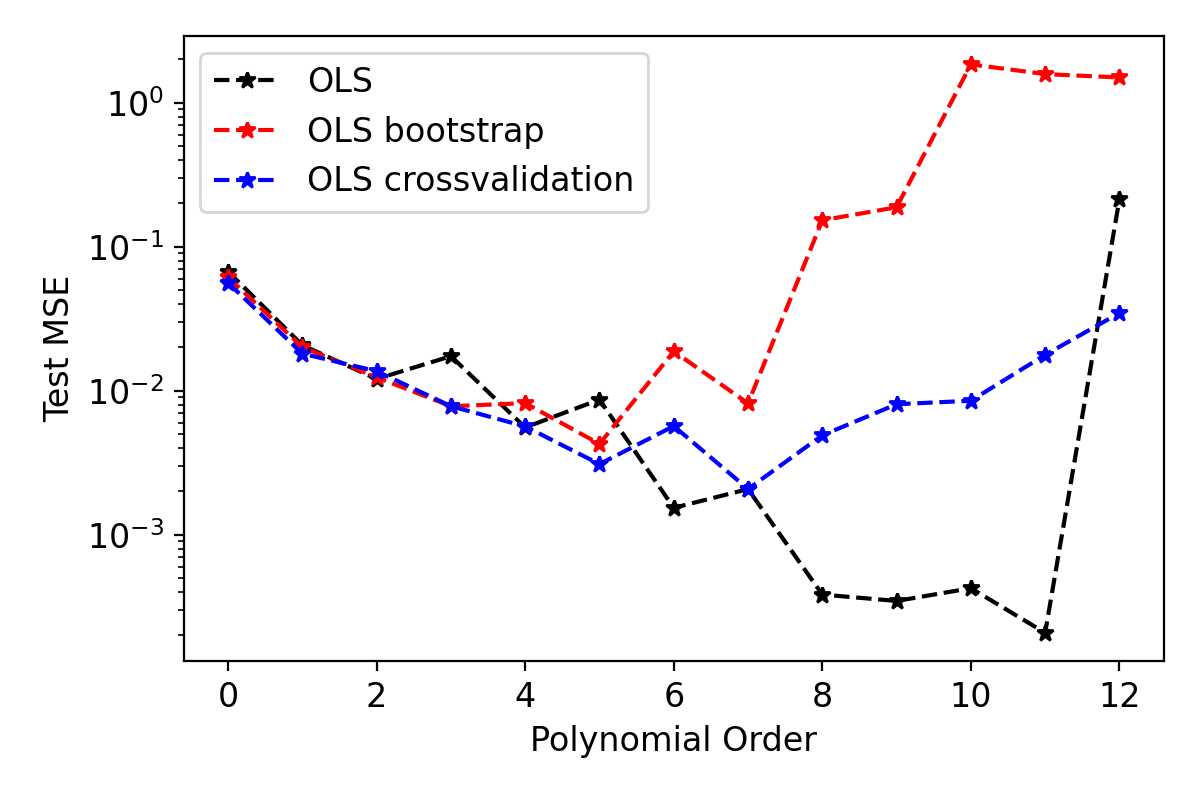
\includegraphics[width=.8\linewidth]{Images/ols14.png}
  \caption{}
  \label{fig:ols14}
\end{subfigure}
\caption{For $r=0.1$, $var=0$ and $n=100$: (a) $MSE_{train}$ and (b) $MSE_{test}$ plotted as functions of model complexity}
\label{fig:OLS_resample2}
\end{figure}

The figure \ref{fig:OLS_resample} shows the comparison between OLS, Ridge, and LASSO methods with bootstrap and cross-validation resampling. Resampling is primarily performed to reduce the variance in statistics like the mean squared error. Often, statistics of a single fit might not be the best indicator of the performance of the model. However, we see that in the case of OLS, introduction of resampling has almost no effect. This can be attributed to the fact that due to $n = 900$, the model 'sees' a variety of data during the training phase. If the number of data points is reduced for example to $n=100$ (see figure \ref{fig:OLS_resample2}), then the effect of resampling is more prominent. We see that for $n=100$, the training is equally well for OLS and OLS with cross-validation resampling. But, $MSE_{train}$ is lower for bootstrap for high values of $p$. This is an indicator of overfitting where, in bootstrap resampling, some of the data is 'seen' again due to sampling with replacement. This reduces the effective training set size and makes the model more prone to overfitting. This is reflected in poor $MSE_{test}$ for OLS with bootstrap resampling. We also think that OLS with cross-validation resampling provides more reliable statistics than OLS without resampling as statistics of OLS with cross-validation can be thought of as a numerical average of statistics of multiple instances of OLS without resampling. The introduction of resampling in Ridge and LASSO has no effect on training (figures \ref{fig:ridge9} and \ref{fig:lasso9}) but they do smoothen out the irregularities of the $MSE_{test}$ (figures \ref{fig:ridge8} and \ref{fig:lasso8}).


\subsubsection{OLS with Stochastic Gradient Descent}
For stochastic gradient descent we have three additional parameters: the epoch $e$, learning rate $\eta$, and the number of mini-batches $n_{batch}$. In their work \cite{masters_revisiting_2018} showed that using small batch sizes achieves the best training stability and test performance across a wide range of experiments. The best results were obtained for batch sizes equal to or smaller than 32. Therefore, we focus in this discussion on batch sizes 1, 2, 5, 10, 32. For a batch size of 1, we have a classical stochastic gradient descent. Otherwise, the algorithm is called mini-batch gradient descent. Usually, the number of epochs is large to sufficiently minimize the error by the learning algorithm. Therefore, we compare the output with epochs of size 10, 100, 500, 1000. Lastly, the learning rate is a small positive number and traditionally between 0 and 1. We analyze the output with the following learning rates 0.001, 0.01, 0.1, 1.0. \newline \newline
While the MSE for the training dataset hardly varies for different learn rates, number of epochs or batch sizes the MSE for the test dataset improves slightly if the parameters are chosen correctly and the order of the fitted polynomial is high (see figure \ref{fig:ols_sgd}). The best results for $MSE_test$ were obtained for $n_{batch}=10, n_e=32$ and $\eta=0.1$. But even for the size of the mini batches, which displays the "biggest" variance in the $MSE_{test}$, the difference is only between roughly $10^{-3}$ and $10^{-4}$ (see figure \ref{fig:olssg_test_batch}). To conclude, the choice of the SGD parameters, which we tested, does not seem to play an important part for the performance of the fitting in this case.

\begin{figure}[H]
\centering
\begin{subfigure}{.49\textwidth}
  \centering
  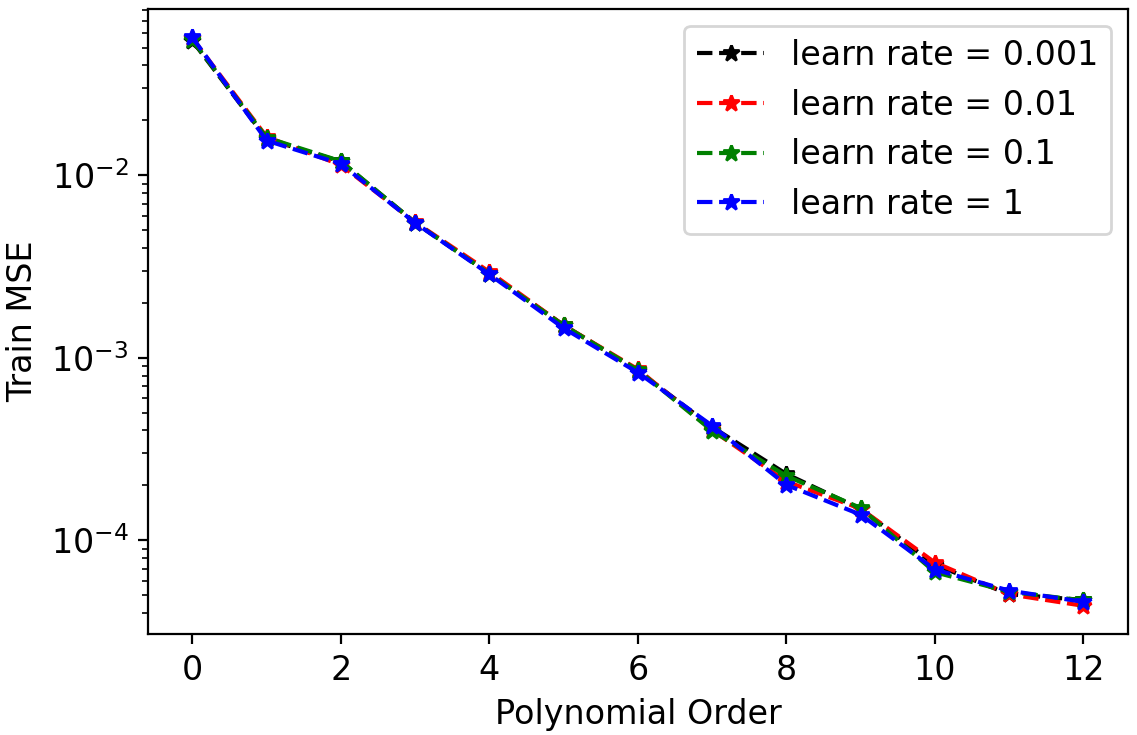
\includegraphics[width=.9\linewidth]{Images/olssgd_train_learn_rate_all_batch_32_epoch_10.png}
  \caption{}
  \label{fig:olssgd_train_learn_rate}
\end{subfigure}%
\begin{subfigure}{.49\textwidth}
  \centering
  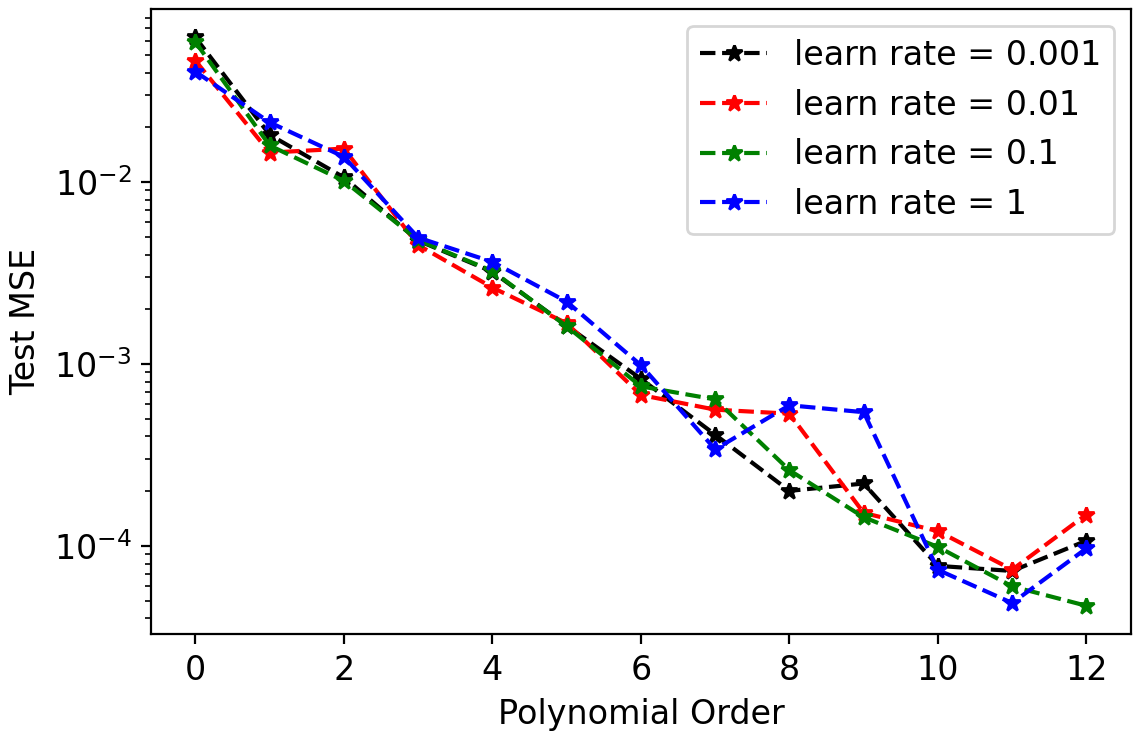
\includegraphics[width=.9\linewidth]{Images/olssgd_test_learn_rate_all_batch_32_epoch_10.png}
  \caption{}
  \label{fig:olssgd_test_learn_rate}
\end{subfigure}
\begin{subfigure}{.49\textwidth}
  \centering
  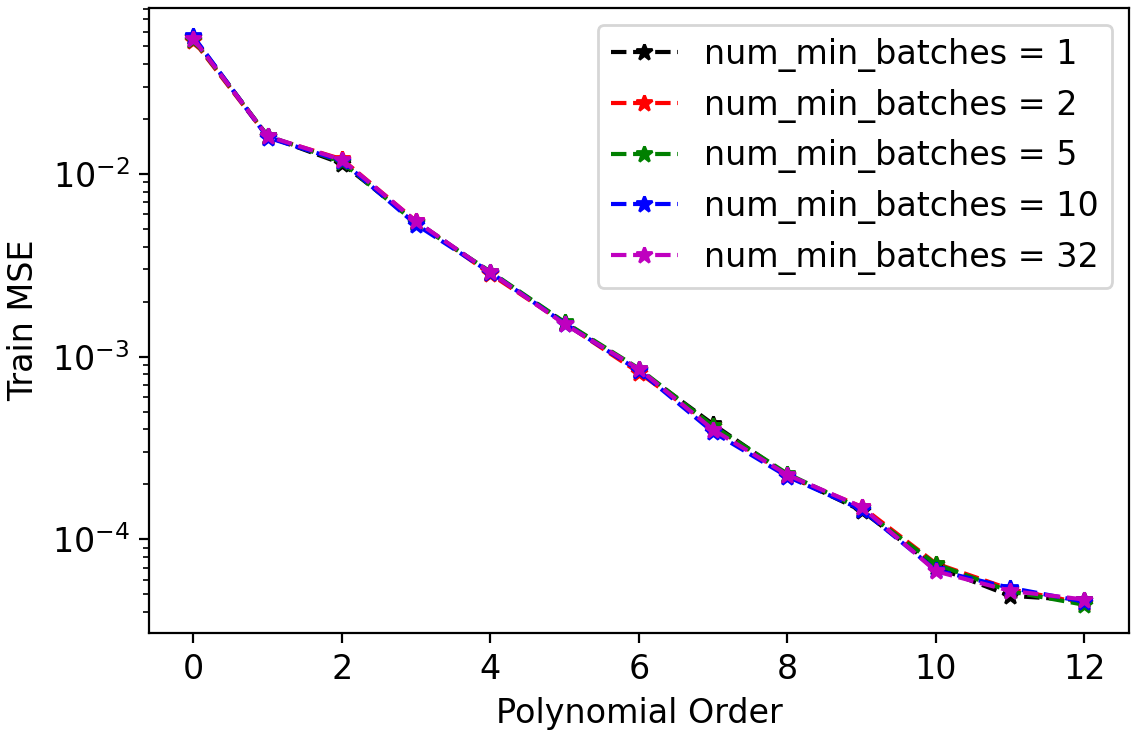
\includegraphics[width=.9\linewidth]{Images/olssgd_train_learn_rate_1_batch_all_epoch_10.png.png}
  \caption{}
  \label{fig:olssgd_train_batch}
\end{subfigure}
\begin{subfigure}{.49\textwidth}
  \centering
  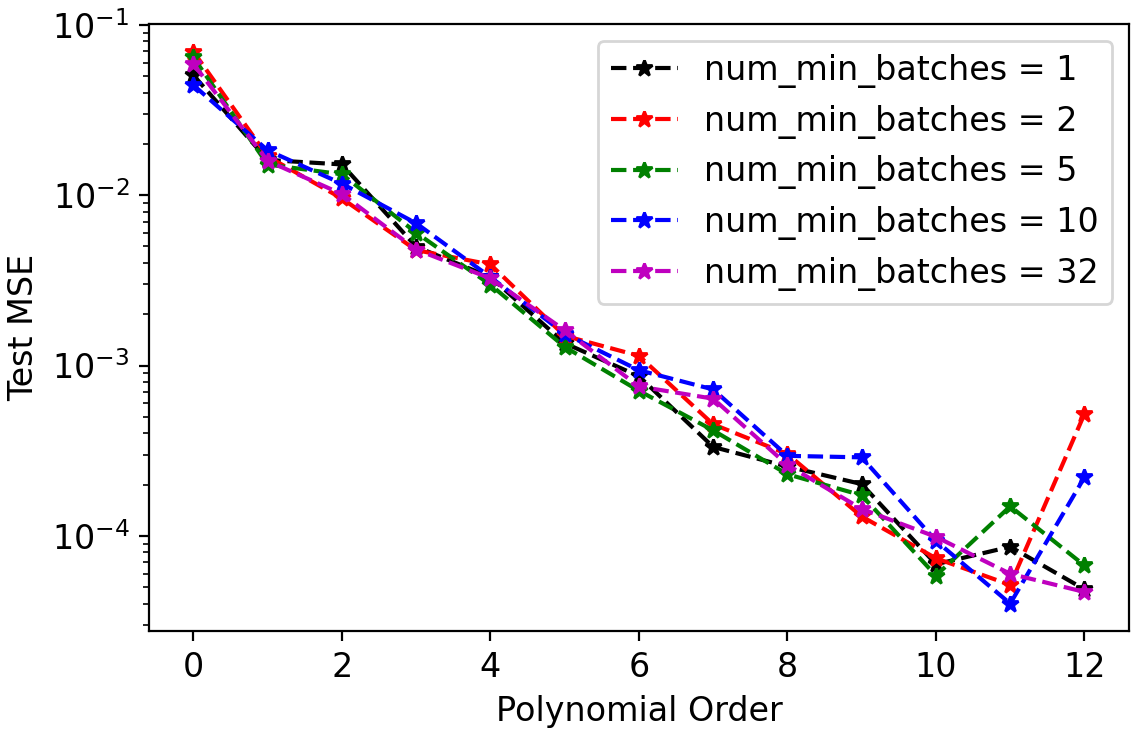
\includegraphics[width=.9\linewidth]{Images/olssgd_test_learn_rate_1_batch_all_epoch_10.png}
  \caption{}
  \label{fig:olssg_test_batch}
\end{subfigure}
\begin{subfigure}{.49\textwidth}
  \centering
  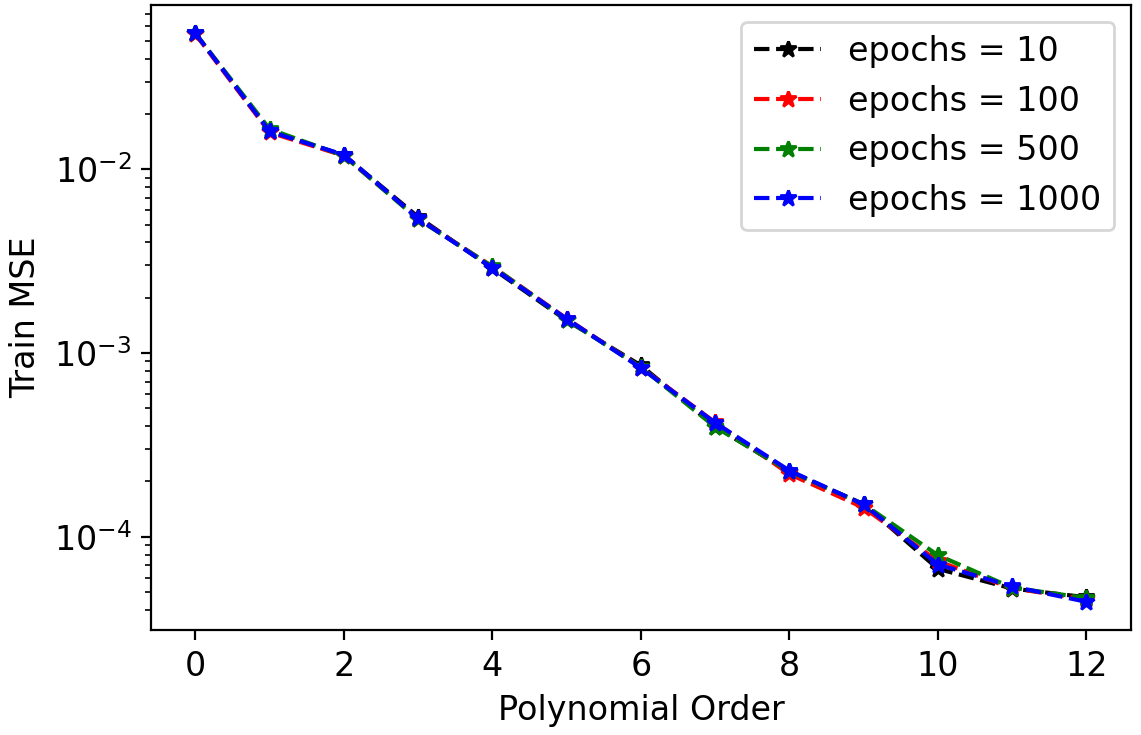
\includegraphics[width=.9\linewidth]{Images/olssgd_train_learn_rate_1_batch_32_epoch_all.png}
  \caption{}
  \label{fig:olssgd_train_epoch}
\end{subfigure}
\begin{subfigure}{.49\textwidth}
  \centering
  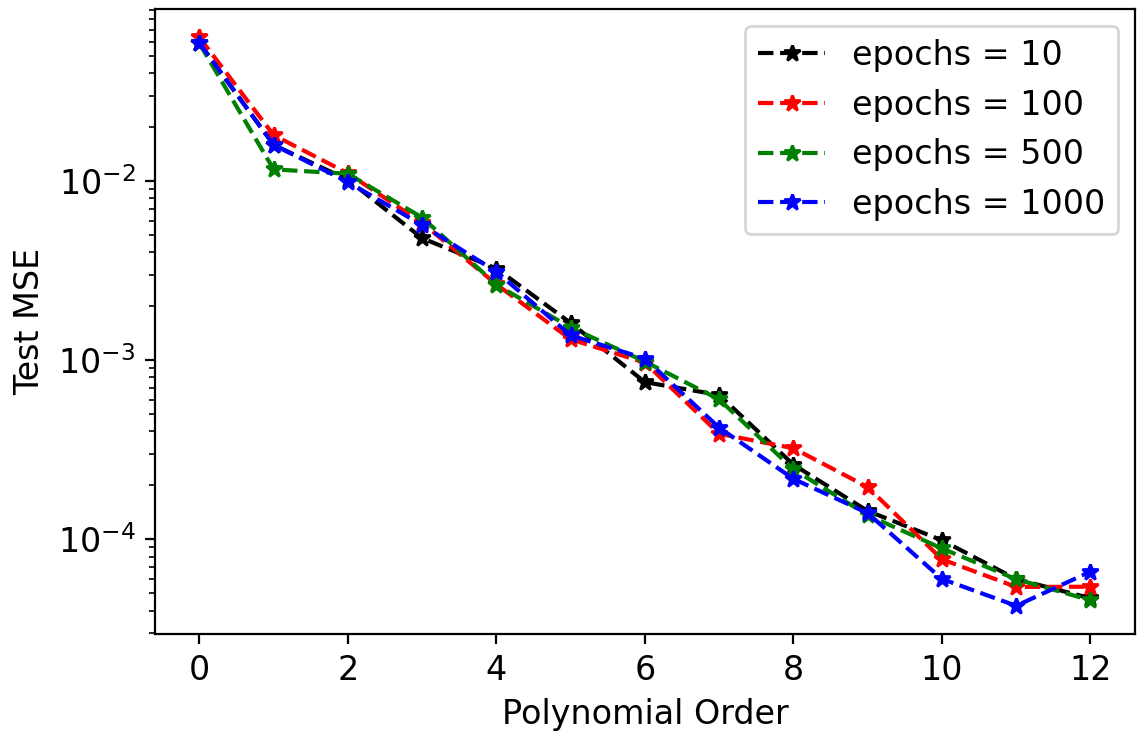
\includegraphics[width=.9\linewidth]{Images/olssgd_test_learn_rate_1_batch_32_epoch_all.png}
  \caption{}
  \label{fig:olssgd_test_epoch}
\end{subfigure}
\caption{For $r=0.1$, $var=0$, $n=900$: $MSE_{train}$ (left column) and $MSE_{test}$ (right column) plotted as functions of model complexity. a), b): $n_{batch}=10, n_e=32$, c), d): $\eta=0.1, n_e=10$, e), f): $\eta=0.1, n_{batch}=32$}
\label{fig:ols_sgd}
\end{figure}
Similar results were also obtained for optimizing the cost function for ridge regression. When we compare the test and train MSE for ridge and OLS regression with and without SGD (see figure \ref{fig:ols_sgd_ridge}) we clearly see that for OLS there is nearly no difference if the mini-batch stochastic gradient descent is applied or not. In contrary, when we look at ridge regression both the train and test MSE are better without applying the mini-batch stochastic gradient descent. For this simulation we used:  $n_{batch}=10, n_e=32, \eta=0.1$ and $\lambda_{ridge}=0.0001$. 
\begin{figure}[H]
	\centering
	\begin{subfigure}{.5\textwidth}
		\centering
		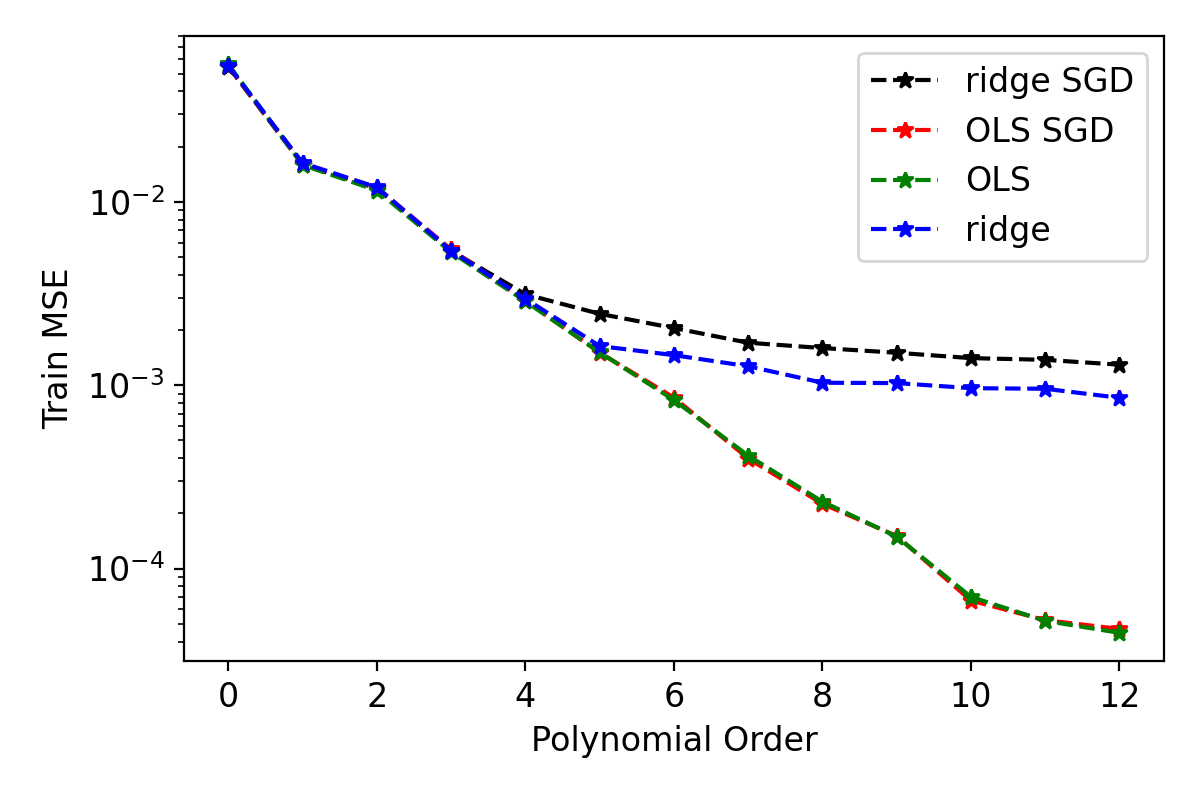
\includegraphics[width=.9\linewidth]{Images/sgd_ols_ridge_train.png}
		\caption{}
		\label{fig:ols_sgd_ridge_train}
	\end{subfigure}%
	\begin{subfigure}{.5\textwidth}
		\centering
		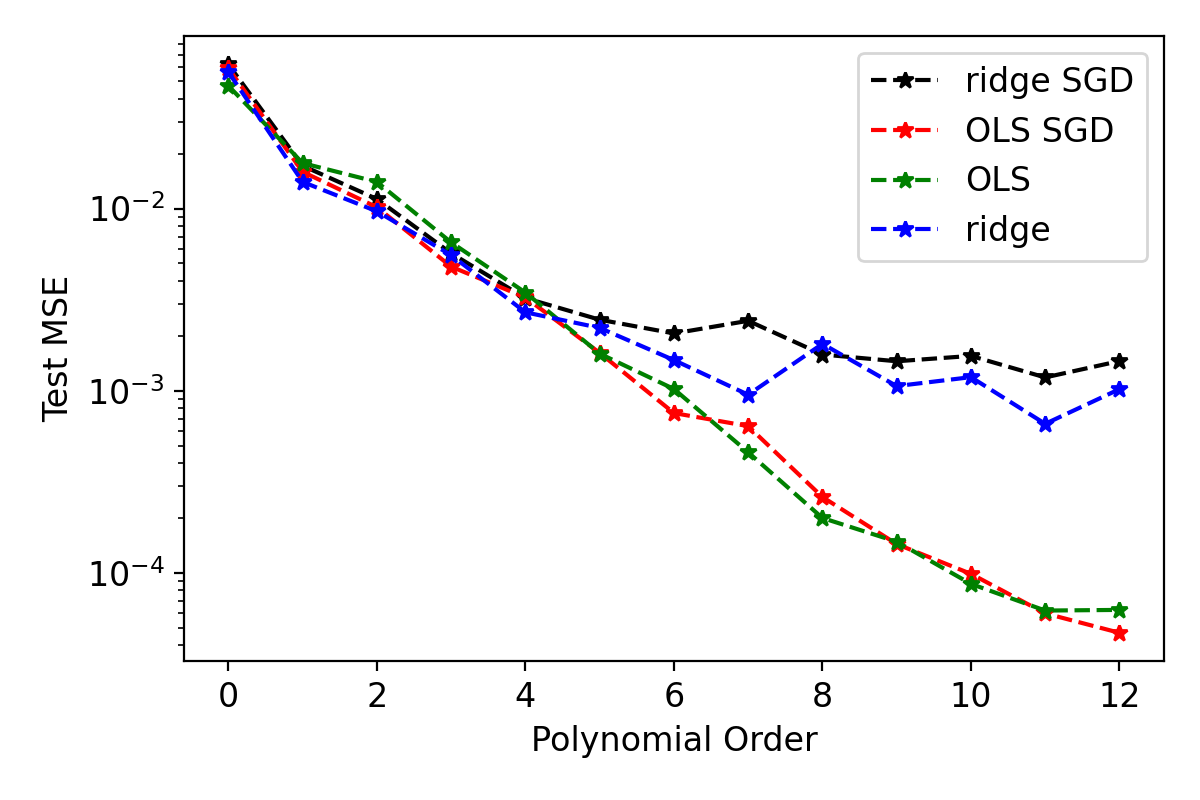
\includegraphics[width=.9\linewidth]{Images/sgd_ols_ridge_test.png}
		\caption{}
		\label{fig:ols_sgd_ridge_test}
	\end{subfigure}
	\caption{For $r=0.1$, $var=0$, $n=900$: $MSE_{train}$ and $MSE_{test}$ plotted as functions of model complexity.}
	\label{fig:ols_sgd_ridge}
\end{figure}

\section{Classification} \label{sec:logistic_regression}
\subsection{Method} \label{subsec:method_logistic_regression}
Linear regression can be extended to classification by two changes \cite{murphy_machine_2012}. First is the change of the Gaussian distribution for $y$ with a Bernoulli distribution, a more appropriate for the case of binary response, $y \in \{0,1\}$. 

$$
p(y \mid \mathbf{x}, \theta)=Ber(y|\mu(x))) = p^k(1-p)^k$$ 

Second is to pass the linear combination of the inputs to a function that ensures $0 \leq \mu(x)\leq 1$. This is achieved by using a logit function also known as sigmoid function, $\mu(x) = sigm(\mathbf{w^T x})$. 

We define,
$$
sigm(z ) = \frac{1}{1 + e^{-z}}
$$

Putting these two steps together we get,
$$
p(y \mid \mathbf{x}, \theta)=Ber(y|sigm(\mathbf{w^T x})))
$$
The negative log-likelihood for logistic regression is given by, 
$$
\begin{aligned}\mathrm{NLL}(\mathbf{w}) &=-\sum_{i=1}^{N} \log \left[\mu_{i}^{\mathrm{I}\left(y_{i}=1\right)} \times\left(1-\mu_{i}\right)^{\mathrm{I}\left(y_{i}=0\right)}\right] \\&=-\sum_{i=1}^{N}\left[y_{i} \log \mu_{i}+\left(1-y_{i}\right) \log \left(1-\mu_{i}\right)\right]\end{aligned}
$$

Unlike linear regression, we can no longer write down the MLE in closed form, thus we need an optimization algorithm to compute it. The simplest algorithm for unconstrained optimization is gradient descent, also known as steepest descent. This is written as follows,

$$\beta_{k+1} = \beta_k - \eta_k g_k$$

where $\eta_k$ is the learning rate and $g_k$ is the gradient of the loss function. There are limitations of gradient descent. It can get stuck in a local minima, it is sensitive to initial condition, and for large dataset it is computationally expensive \cite{mehta2019high}. This can be overcome by adding stochasticity, for instance, by only taking the gradient of a subset of data called mini-batches. 

\subsubsection{Stochastic Gradient descent with mini-batches}
If there are n samples in total, and the mini-batch size set is M, there are n/M possible mini-batches $B_k $ where $k \in (1,2,..n/M)$. In this case, the gradient descent in each cycle over the mini batches is approximated by using a single mini-batch. The approximated gradient descent over a single batch is then used as a gradient in the update of the parameter. We denote the approximated gradient by, 
$$
\nabla_{\beta} C^{MB}(\beta) = \sum_{i\in B_k} \nabla_\beta c_i(\textbf{x}_i, \theta)
$$

The SGD with mini-batches equation is given by, 
$$
g_k = \eta \nabla_{\beta} C^{MB}(\beta) \\
\beta_{k+1} = \beta_k - g_k
$$

\subsubsection{Support Vector Machine}\label{subsubsec:SVM}

\subsection{Data} \label{subsec:data_logistic_regression}
For logistic regression and Support Vector Machines, we use the Wisconsin Breast Cancer Dataset \footnote{\url{https://www.kaggle.com/uciml/breast-cancer-wisconsin-data}}. This dataset contains measurements for breast cancer cases. There are two types of cancer in the dataset benign and malignant. An overview of the dataset if given in the jupyter notebook \href{https://github.com/am-kaiser/CompSci-Project-1/blob/main/regression_analysis/examples/logistic_regression_analysis.ipynb}{logistic\_regression\_analysis} which can be found in the GitHub repository corresponding to this report. Based on this dataset we want to find a model which predicts the diagnosis, i.e. either benign or malignant. For the design matrix, we drop the column id and diagnosis from the data. The id is not important for making predictions and the diagnosis is what we want to predict.
\subsection{Results} \label{subsec:results_logistic_regression}

\section{Summary} \label{sec:summary}

We trained various linear regression models like OLS, ridge, and lasso to fit polynomials to the Franke function with noise. Thereafter, we used the model to predict the output for unseen test data. Various statistics like $MSE$, $R^2$ Error, and generalization error were used to probe the model performance. We also applied resampling techniques to reduce the uncertainty in the statistics. Along with finding optimal parameters directly using closed-form solutions, we also utilized stochastic gradient descent to find optimal parameters. We discovered that OLS is better at predicting than lasso and ridge for the sample data considered. When the lasso and ridge models tend to more OLS like behavior i.e. $\lambda_l$ and $\lambda_r$ tend to 0, the prediction improves. OLS performed several orders of magnitude better than lasso regression and a few orders of magnitude better than ridge in terms of the prediction error. We also experienced the problem of overfitting when the training data was less numerous and particularly during bootstrap resampling where the effective data that the model could 'see' during the training phase was reduced due to sampling with replacement. \newline
In addition, we used logistic regression and Support Vector Machines to fit a model to the Wisconsin Breast Cancer data. Overall, we showed that SVM with a linear kernel is the best performing classification algorithm for this setup. Nonetheless, all tested methods performed well when classifying benign classes. While the performance could be improved for malignant ones.

\section{Acknowledgement} \label{subsec:acknowledgement}
All contributors to this report are part of the \href{https://www.mn.uio.no/compsci/english/}{CompSci} doctoral program which is managed by the Faculty of Mathematics and Natural Sciences at the University of Oslo (UiO).
The program is partly funded by the EU Horizon 2020 under the Marie Skłodowska-Curie Action (MSCA) - Co-funding of Regional, National and International Programmes (COFUND).
%------------------------------------------------------------------------
\newpage
\bibliographystyle{plain} 
\bibliography{references}
\end{document}
